\documentclass{tufte-book}

\title{CSC499 Honors Class \\Project Report \\Template}
\author[T]{Yang Ho and Johnny Nguyen, under the
tutelage of Dr. Franc Brglez, 
Computer Science, NCSU}
\publisher{Publishers of This Report}

%%%%% from Franc Brglez
\newcommand{\labs}{\texttt{labs}}
\newcommand{\coordUpdate}{\texttt{coordUpdate}}
\newcommand{\lMAts}{\texttt{lMAts}}
\newcommand{\lssMAts}{\texttt{lssMAts}}
\newcommand{\lssRRts}{\texttt{lssRRts}}
\newcommand{\lssOrel}{\texttt{lssOrel}}
\newcommand{\lssOrelU}{\texttt{lssOrel\_{U}}}
\newcommand{\lssOrelE}{\texttt{lssOrel\_{8}}}
\newcommand{\lssMAtsE}{\texttt{lssMAts\_{8}}}

%%%%%%%%%% From Borko
\usepackage{amssymb}
\usepackage{algorithm}
\usepackage{algorithmic}

\newcommand{\valueBest}{$\Theta({\underline{\varsigma}}^{*})$}
\newcommand{\valueTarget}{$\Theta^{ub}_{L}$}
\renewcommand{\algorithmicbody}{}
\newcommand{\CALL}[2]{\texttt{{#1}(#2)}}
\newcommand{\PROCEDURE}[1]{%
	\renewcommand{\algorithmicwhile}{\textbf{procedure}}
	\renewcommand{\algorithmicdo}{ }
	\WHILE{#1}
	\renewcommand{\algorithmicwhile}{\textbf{while}}
	\renewcommand{\algorithmicdo}{\textbf{do}}	
}
\newcommand{\ENDPROCEDURE}{\ENDWHILE}
\renewcommand\algorithmiccomment[1]{\hfill $\vartriangleright$ #1 }
\floatstyle{plain}
\newfloat{myalgo}{tbhp}{mya}

\newenvironment{algorithm-wide}[2][tbh]%
{\begin{myalgo}[#1]
\centering
\begin{minipage}{#2}
\begin{algorithm}[H]}%
{\end{algorithm}
\end{minipage}
\end{myalgo}}

\definecolor{Gray}{rgb}{0.9,0.9,0.9}

\setcounter{secnumdepth}{ 1} % { 1} to get BOTH chapters and sections numbered 
                             % { 0} to get only chapters numbered
                             % {-1} to turn off all numbering
\begin{document}

\maketitle
% v.4 copyright page
\newpage
\begin{fullwidth}
~\vfill
\thispagestyle{empty}
\setlength{\parindent}{0pt}
\setlength{\parskip}{\baselineskip}
Copyright \copyright\ \the\year\ \thanklessauthor

\par\smallcaps{Published by \thanklesspublisher}

\par\smallcaps{tufte-latex.googlecode.com}

\par Licensed under the Apache License, Version 2.0 (the ``License''); you may not
use this file except in compliance with the License. You may obtain a copy
of the License at \url{http://www.apache.org/licenses/LICENSE-2.0}. Unless
required by applicable law or agreed to in writing, software distributed
under the License is distributed on an \smallcaps{``AS IS'' BASIS, WITHOUT
WARRANTIES OR CONDITIONS OF ANY KIND}, either express or implied. See the
License for the specific language governing permissions and limitations
under the License.\index{license}

\par\textit{First printing, \monthyear}
\end{fullwidth}

\newpage
\chapter*{Summary}
\vspace*{-4ex}
\newthought{This report}\sidenote{The
template for this report is based on an eBook template 
at~\url{https://github.com/fbrglez/gitPublic/tree/master/xLatex} which itself is a derivate of the Tufte Book Template 
which can be accessed
at~\url{https://github.com/Tufte-LaTeX/tufte-latex} 
} 
summarizes our work on the project
with a working title of 
{\em On Rapid Prototyping of Combinatorial Solvers}.
\par
As a prerequisite, we have installed the {\em R} shell, the {\em tcl/TkCon} shell, the {\em python} shell, and various \LaTeX\ templates. The default working shell is
{\em bash} under linux for Yang Ho and {\em bash} under MacOSX for Johnny Nguyen.
The files shared in the project are accessible on  
GitHub\cite{Lib-OPUS2-gitPublic-Brglez}.
%GitHub\cite{Lib-OPUS-xBed-2015-gitPublic-Brglez}.
%\footnote{See {\color{blue} \url{https://github.com/fbrglez/gitPublic/}}.
All of the initial prototypes of combinatorial solvers are written in tcl and
are introduced, with required tcl commands and test cases, during the weekly class meeting by the instructor. There are several goals of this project. First, we observe the behaviour and learn about properties of each solver in real time
by executing tcl commands and modifying the tcl code, rather than study the pseudo code in 
the abstract. Second, we learn about python to construct a solver that is comparable to
the tcl implementation, not only in consiseness and clarity but most importanly, may well exceed the runtime performance of the tcl solver. Third, we instrument each solver
for performance evaluation on a large number of instances running on the same CPU, so we can infer performance differences between solvers that are statistically significant.
\par
Our current work involves two combinatorial solvers:
one solves the {\em lightout puzzle}, one solves the {\em linear ordering problem}.
The various phases of this project are summarized into sections as outlined
under {\em Contents} 
below\footnote{Note that each line in the ``Contents'' also represents a hyperlink to the respective section and subsection.}.
 
\newthought{And now,} filler text with command \verb+\lipsum[2]+.
\lipsum[2]

% r.5 contents
\tableofcontents
\listoffigures
\listoftables
\listofalgorithms
% Start the main matter (normal chapters)
\mainmatter

\chapter{About Text Items}
\label{chap-About}
\newthought{Text items in this chapter} are divided into three sections:

(1) about notational conventions and schema of \LaTeX~files,

(2) text items selected from Tufte's book template,

(3) text items from other sources,

(4) typesetting examples of algorithms.

\newthought{For details} about how figures and tables are being represented,
see Chapters~\ref{chap-Figures} and~\ref{chap-Tables}.
For additional examples of algorithms, see Chapter~\ref{chap-Algorithms2}.

\clearpage
\section{About Notational Conventions and Schema for \LaTeX~ files}
\label{chap-About-Conventions}

\newthought{When collaborating} with multiple authors using \LaTeX,
conventions about notation and file structures
will save a lot of time.
The schema in Figure~\ref{fg-latex-conventions} already illustrates
a number of conventions that are being  used in this document. 
The list below includes not only the items which are in plain sight in Figure~\ref{fg-latex-conventions}, it also includes items we can observe in subdirectories {\em Algorithms, Figures}, and {\em Tables} as well as the *.tex files in these subdirectories.
\begin{marginfigure}[13ex]%
  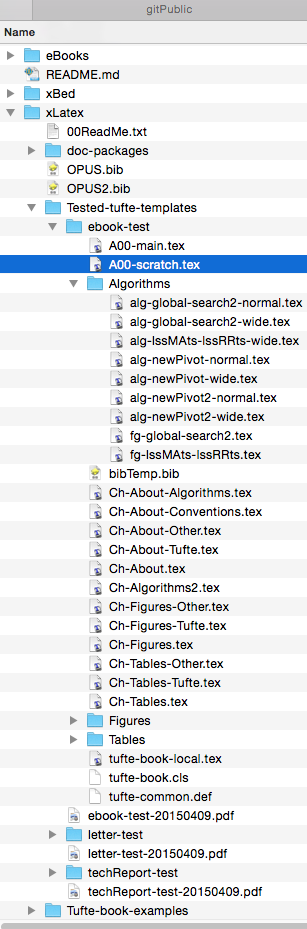
\includegraphics[width=\linewidth]{fg-latex-conventions}
  \caption[Example file fg-latex-conventions.tex]
  {Notational conventions and schema for \LaTeX~files to support collaboration.}
  \label{fg-latex-conventions}
\end{marginfigure}.
%\clearpage
%\small{
\begin{itemize}
\item
Consistently avoid file names with {\em underscore} (\verb+_+).
\item
For complex algorithms, figures and tables, create a separate file which is
prefixed with either \verb+alg-+, \verb+fg-+ or \verb+tb-+
and move the file into the designated subdirectory.
Use the rootname of the file for the label that is used to reference the 
algorithm, figure, or table. For example, we can thus refer to 
contents of file alg-global-search2-normal.tex as 
\verb+Algorithm~\ref{alg-global-search2-normal}+.
Notably, we embed contents of algorithm not only under
\verb+\algorithm+, \verb+\algorithm-wide+ environments but also under 
\verb+\figure+, \verb+\figure*+ environments.
\item
There is always the easy-to-find-file \verb+A00-main.tex+.
This file not only invokes \verb+\documentclass{tufte-book}+
and  the supporting files *tufte*, but also all 
items that are generic to the layout of the book and
new command defitions that are  content-specific with respect to the book.
Finaly, this file also
invokes the book chapters in a well-defined sequence such as 
Ch-About.tex, Ch-Figures.tex, Ch-Tables.tex, and Ch-Algorithms2.tex.
The amount of text in a typical chapter will rarely extend beyond a single page 
since each chapter is likely to invoke
a number of sections that reside in adjacent files and
may represent contributions from several collaborating authors. 
For example, Ch-About.tex invokes four files in this order:
 Ch-About-Conventions.tex,  Ch-About-Tufte.tex, 
  Ch-About-Other.tex,  Ch-About-Algorithms.tex.
\item
The only  *.bib file in the directory ebook-test, bibTemp.bib,
is initially an empty file. 
Within the file \verb+A00-main.tex+, we use relative paths to define
location of the `nearby files' OPUS.bib and OPUS2.bib under xLatex:~
\verb+\bibliography{\detokenize{../../OPUS},+\\
\verb+\detokenize{../../OPUS2}, \detokenize{./bibTemp}}+.\\
Both files, OPUS.bib and OPUS2.bib, are almost always up-to-date
for use by all project participants, so the need for
temporary bib items under the file bibTemp.bib seldom arises.

\end{itemize}
%}
\clearpage
\section{Text Items Selected from Tufte's Book Template}
\label{chap-About-Tufte}

\newthought{The primary text items} for this section are selections
from Tufte Book Template\sidenote{The Tufte Book Template can be accessed
at~\url{https://github.com/Tufte-LaTeX/tufte-latex}.}
Here, we extracted three sections from the Chapter on
{\em On the Use of the tufte-book Document Class}:
From this template, have extracted three sections
\begin{itemize}
\item Page Layout: Headings
\item Sidenotes
\item References
\end{itemize}
However, in this document, we treat all of these three sections as subsections. 


\subsection{Page Layout: Headings}\label{sec:headings}\index{headings}

\newthought{Tufte's books} include the following heading levels: parts,
chapters,\sidenote{Parts and chapters are defined for the \texttt{tufte-book}
class only.}  sections, subsections, and paragraphs.  Not defined by default
are: sub-subsections and subparagraphs.

\begin{table}[h]
  \begin{center}
    \footnotesize%
    \begin{tabular}{lcr}
      \toprule
      Heading & Style & Size \\
      \midrule
      Part & roman & \measure{24}{36}{40} \\
      Chapter & italic & \measure{20}{30}{40} \\
      Section & italic & \measure{12}{16}{26} \\
      Subsection & italic & \measure{11}{15}{26} \\
      Paragraph & italic & 10/14 \\
      \bottomrule
    \end{tabular}
  \end{center}
  \caption{Heading styles used in \BE.}
  \label{tab:heading-styles}
\end{table}

\paragraph{Paragraph} Paragraph headings (as shown here) are introduced by
italicized text and separated from the main paragraph by a bit of space.

This style provides \textsc{a}- and \textsc{b}-heads (that is,
\Verb|\section| and \Verb|\subsection|), demonstrated above.

If you need more than two levels of section headings, you'll have to define
them yourself at the moment; there are no pre-defined styles for anything below
a \Verb|\subsection|.  As Bringhurst points out in \textit{The Elements of
Typographic Style},\cite{Bringhurst2005} you should ``use as many levels of
headings as you need: no more, and no fewer.''

The \TL classes will emit an error if you try to use
\linebreak\Verb|\subsubsection| and smaller headings.

% let's start a new thought -- a new section
\newthought{In his later books},\cite{Tufte2006} Tufte
starts each section with a bit of vertical space, a non-indented paragraph,
and sets the first few words of the sentence in \textsc{small caps}.  To
accomplish this using this style, use the \doccmddef{newthought} command:
\begin{docspec}
  \doccmd{newthought}\{In his later books\}, Tufte starts\ldots
\end{docspec}


\subsection{Sidenotes}\label{sec:sidenotes}
One of the most prominent and distinctive features of this style is the
extensive use of sidenotes.  There is a wide margin to provide ample room
for sidenotes and small figures.  Any \doccmd{footnote}s will automatically
be converted to sidenotes.\footnote{This is a sidenote that was entered
using the \texttt{\textbackslash footnote} command.}  If you'd like to place ancillary
information in the margin without the sidenote mark (the superscript
number), you can use the \doccmd{marginnote} command.\marginnote{This is a
margin note.  Notice that there isn't a number preceding the note, and
there is no number in the main text where this note was written.}

The specification of the \doccmddef{sidenote} command is:
\begin{docspec}
  \doccmd{sidenote}[\docopt{number}][\docopt{offset}]\{\docarg{Sidenote text.}\}
\end{docspec}

Both the \docopt{number} and \docopt{offset} arguments are optional.  If you
provide a \docopt{number} argument, then that number will be used as the
sidenote number.  It will change of the number of the current sidenote only and
will not affect the numbering sequence of subsequent sidenotes.

Sometimes a sidenote may run over the top of other text or graphics in the
margin space.  If this happens, you can adjust the vertical position of the
sidenote by providing a dimension in the \docopt{offset} argument.  Some
examples of valid dimensions are:
\begin{docspec}
  \ttfamily 1.0in \qquad 2.54cm \qquad 254mm \qquad 6\Verb|\baselineskip|
\end{docspec}
If the dimension is positive it will push the sidenote down the page; if the
dimension is negative, it will move the sidenote up the page.

While both the \docopt{number} and \docopt{offset} arguments are optional, they
must be provided in order.  To adjust the vertical position of the sidenote
while leaving the sidenote number alone, use the following syntax:
\begin{docspec}
  \doccmd{sidenote}[][\docopt{offset}]\{\docarg{Sidenote text.}\}
\end{docspec}
The empty brackets tell the \Verb|\sidenote| command to use the default
sidenote number.

If you \emph{only} want to change the sidenote number, however, you may
completely omit the \docopt{offset} argument:
\begin{docspec}
  \doccmd{sidenote}[\docopt{number}]\{\docarg{Sidenote text.}\}
\end{docspec}

The \doccmddef{marginnote} command has a similar \docarg{offset} argument:
\begin{docspec}
  \doccmd{marginnote}[\docopt{offset}]\{\docarg{Margin note text.}\}
\end{docspec}

\subsection{References}
References are placed alongside their citations as sidenotes,
as well.  This can be accomplished using the normal \doccmddef{cite}
command.\sidenote{The first paragraph of this document includes a citation.}

The complete list of references may also be printed automatically by using
the \doccmddef{bibliography} command.  (See the end of this document for an
example.)  If you do not want to print a bibliography at the end of your
document, use the \doccmddef{nobibliography} command in its place.  

To enter multiple citations at one location,\cite[-3\baselineskip]{Tufte2006,Tufte1990} you can
provide a list of keys separated by commas and the same optional vertical
offset argument: \Verb|\cite{Tufte2006,Tufte1990}|.  
\begin{docspec}
  \doccmd{cite}[\docopt{offset}]\{\docarg{bibkey1,bibkey2,\ldots}\}
\end{docspec}
\clearpage
%\chapter{About Text Items}
%\label{chap-About}
%\newthought{Text items in this chapter} are divided into two sections: 
%(1) test items from Tufte,
%(2) test items  from other sources.
%
%\newthought{For details} about how figures and tables are being represented,
%see Chapters~\ref{chap-Figures} and~\ref{chap-Tables}.
%
%\section{Text Items Selected from Tufte's Book Template}
\label{chap-About-Tufte}

\newthought{The primary text items} for this section are selections
from Tufte Book Template\sidenote{The Tufte Book Template can be accessed
at~\url{https://github.com/Tufte-LaTeX/tufte-latex}.}
Here, we extracted three sections from the Chapter on
{\em On the Use of the tufte-book Document Class}:
From this template, have extracted three sections
\begin{itemize}
\item Page Layout: Headings
\item Sidenotes
\item References
\end{itemize}
However, in this document, we treat all of these three sections as subsections. 


\subsection{Page Layout: Headings}\label{sec:headings}\index{headings}

\newthought{Tufte's books} include the following heading levels: parts,
chapters,\sidenote{Parts and chapters are defined for the \texttt{tufte-book}
class only.}  sections, subsections, and paragraphs.  Not defined by default
are: sub-subsections and subparagraphs.

\begin{table}[h]
  \begin{center}
    \footnotesize%
    \begin{tabular}{lcr}
      \toprule
      Heading & Style & Size \\
      \midrule
      Part & roman & \measure{24}{36}{40} \\
      Chapter & italic & \measure{20}{30}{40} \\
      Section & italic & \measure{12}{16}{26} \\
      Subsection & italic & \measure{11}{15}{26} \\
      Paragraph & italic & 10/14 \\
      \bottomrule
    \end{tabular}
  \end{center}
  \caption{Heading styles used in \BE.}
  \label{tab:heading-styles}
\end{table}

\paragraph{Paragraph} Paragraph headings (as shown here) are introduced by
italicized text and separated from the main paragraph by a bit of space.

This style provides \textsc{a}- and \textsc{b}-heads (that is,
\Verb|\section| and \Verb|\subsection|), demonstrated above.

If you need more than two levels of section headings, you'll have to define
them yourself at the moment; there are no pre-defined styles for anything below
a \Verb|\subsection|.  As Bringhurst points out in \textit{The Elements of
Typographic Style},\cite{Bringhurst2005} you should ``use as many levels of
headings as you need: no more, and no fewer.''

The \TL classes will emit an error if you try to use
\linebreak\Verb|\subsubsection| and smaller headings.

% let's start a new thought -- a new section
\newthought{In his later books},\cite{Tufte2006} Tufte
starts each section with a bit of vertical space, a non-indented paragraph,
and sets the first few words of the sentence in \textsc{small caps}.  To
accomplish this using this style, use the \doccmddef{newthought} command:
\begin{docspec}
  \doccmd{newthought}\{In his later books\}, Tufte starts\ldots
\end{docspec}


\subsection{Sidenotes}\label{sec:sidenotes}
One of the most prominent and distinctive features of this style is the
extensive use of sidenotes.  There is a wide margin to provide ample room
for sidenotes and small figures.  Any \doccmd{footnote}s will automatically
be converted to sidenotes.\footnote{This is a sidenote that was entered
using the \texttt{\textbackslash footnote} command.}  If you'd like to place ancillary
information in the margin without the sidenote mark (the superscript
number), you can use the \doccmd{marginnote} command.\marginnote{This is a
margin note.  Notice that there isn't a number preceding the note, and
there is no number in the main text where this note was written.}

The specification of the \doccmddef{sidenote} command is:
\begin{docspec}
  \doccmd{sidenote}[\docopt{number}][\docopt{offset}]\{\docarg{Sidenote text.}\}
\end{docspec}

Both the \docopt{number} and \docopt{offset} arguments are optional.  If you
provide a \docopt{number} argument, then that number will be used as the
sidenote number.  It will change of the number of the current sidenote only and
will not affect the numbering sequence of subsequent sidenotes.

Sometimes a sidenote may run over the top of other text or graphics in the
margin space.  If this happens, you can adjust the vertical position of the
sidenote by providing a dimension in the \docopt{offset} argument.  Some
examples of valid dimensions are:
\begin{docspec}
  \ttfamily 1.0in \qquad 2.54cm \qquad 254mm \qquad 6\Verb|\baselineskip|
\end{docspec}
If the dimension is positive it will push the sidenote down the page; if the
dimension is negative, it will move the sidenote up the page.

While both the \docopt{number} and \docopt{offset} arguments are optional, they
must be provided in order.  To adjust the vertical position of the sidenote
while leaving the sidenote number alone, use the following syntax:
\begin{docspec}
  \doccmd{sidenote}[][\docopt{offset}]\{\docarg{Sidenote text.}\}
\end{docspec}
The empty brackets tell the \Verb|\sidenote| command to use the default
sidenote number.

If you \emph{only} want to change the sidenote number, however, you may
completely omit the \docopt{offset} argument:
\begin{docspec}
  \doccmd{sidenote}[\docopt{number}]\{\docarg{Sidenote text.}\}
\end{docspec}

The \doccmddef{marginnote} command has a similar \docarg{offset} argument:
\begin{docspec}
  \doccmd{marginnote}[\docopt{offset}]\{\docarg{Margin note text.}\}
\end{docspec}

\subsection{References}
References are placed alongside their citations as sidenotes,
as well.  This can be accomplished using the normal \doccmddef{cite}
command.\sidenote{The first paragraph of this document includes a citation.}

The complete list of references may also be printed automatically by using
the \doccmddef{bibliography} command.  (See the end of this document for an
example.)  If you do not want to print a bibliography at the end of your
document, use the \doccmddef{nobibliography} command in its place.  

To enter multiple citations at one location,\cite[-3\baselineskip]{Tufte2006,Tufte1990} you can
provide a list of keys separated by commas and the same optional vertical
offset argument: \Verb|\cite{Tufte2006,Tufte1990}|.  
\begin{docspec}
  \doccmd{cite}[\docopt{offset}]\{\docarg{bibkey1,bibkey2,\ldots}\}
\end{docspec}
%%\chapter{About Text Items}
%\label{chap-About}
%\newthought{Text items in this chapter} are divided into two sections: 
%(1) test items from Tufte,
%(2) test items  from other sources.
%
%\newthought{For details} about how figures and tables are being represented,
%see Chapters~\ref{chap-Figures} and~\ref{chap-Tables}.
%
%\input{Ch-About-Tufte}
%\input{Ch-About-Other}
\section{About Text Items from Other Sources}
\label{chap-About-Other}

\newthought{The primary text items} for this section are selections
from\cite[-1ex]{Lib-OPUS2-labs-2015-arxiv-Boskovic}.

\vspace*{1.5ex}\noindent
The command \verb+\cmt+ as listed below,
\cmt{creates a `comment' sentence like this one.}\\  
\verb+\newcommand{\cmt}[1]{\textsf{[#1]}}+

\vspace*{1.5ex}\noindent
The command \verb+\OMIT+ as listed below\\
\verb+\newcommand{\OMIT}[1]{}+ \\
suppresses a block of text listed in the latex source code below
(it makes it invisible).
\OMIT{
\TOPIC{Local paragraph} 
This boldface {\em Local paragraph.} has been created by using 
the local command \verb+\TOPIC+: see the command below\\
\verb+\newcommand{\TOPIC}[1]{\vspace{1.3ex}\par\noindent\textbf{#1.}}+
}

\TOPIC{Local paragraph} 
This boldface headings, terminated with a period, {\em Local paragraph.} has been created by using 
the local command \verb+\TOPIC+: see the command below\\
\verb+\newcommand{\TOPIC}[1]{\vspace{1.3ex}\par\noindent\textbf{#1.}}+\\
\noindent
NOTE: such heading may be considered `too bold' in the context of Tufte's ideas in
{\em Beautiful Evidence}.

\paragraph{Tufte's Paragraph} Paragraph headings (as shown here) are introduced by
italicized text and separated from the main paragraph by a bit of space.
The command is \\
\verb+\paragraph{}+


\TOPIC{About the labs problem}
The {\em aperiodic low-autocorrelation binary sequence} (\labs) problem 
has a simple formulation: take a binary sequence of length $L$,  
$S = s_1 s_2 \ldots s_L$, $s_i \in \{ +1,-1 \}$, the autocorrelation function
$C_k(S) = \sum_{i=1}^{L-k}s_{i}s_{i+k},$ and minimize the energy function:
\begin{equation}
E(S) =  \sum_{k=1}^{L-1}C_{k}^{2}(S)
\label{eq_energy}
\end{equation}
or alternatively, maximize the 
{\em merit factor F}\cite[-1ex]{Lib-OPUS-labs-1977-IEEE_TIT-Golay,
Lib-OPUS-labs-1982-IEEE_TIT-Golay,
Lib-OPUS-labs-1990-IEEE_TIT-Golay-skewsym}:
\begin{equation}
F(S) =  {L^2}/({2E(S)}).
\label{eq_meritFactor}
\end{equation}
 

The asymptotic value for the maximum merit factor $F$, introduced
by Golay, has been re-derived
using arguments from statistical mechanics\cite[2ex]{Lib-OPUS-labs-1987-JourPhys-Bernasconi}:
\begin{equation}
{\rm as~~~} L \rightarrow \infty {\rm ,~~~then~~~}F  \rightarrow 12.3248
\label{eq_asymptotic}
\end{equation} 
The publication of the asymptotic value in Eq. \ref{eq_asymptotic}
is providing an on-going challenge since no published solutions can yet claim to converge to this value
as the length of the sequence increases. 

\TOPIC{Creating a filler text}
The remainder of this paragraph has been created with the command \verb+\lipsum[4]+.
\lipsum[4]

%\paragraph{Creating more filler text}
%The remainder of this paragraph has been created with command \verb+\lipsum[1]+.
%\lipsum[1]

\TOPIC{More about the labs problem}
Finding the optimum sequence is significantly harder than solving the special cases of the Ising spin-glass problems with limited interaction and periodic boundary conditions, for 
example\cite{Lib-OPUS-labs-2003-GECCO-Goldberg-periodic}. 
While effective methods have been presented to solve the special 
cases\cite[3ex]{Lib-OPUS-labs-2003-GECCO-Goldberg-periodic}, up to $L = 400$, 
the best merit factors that has also been {\em proven optimal} for the problem as formulated in Eq. \ref{eq_meritFactor}
are presently known for values of $L \le 60$ 
only\cite[3ex]{Lib-OPUS-labs-1996-JPhysA-Mertens-BB_solutions}.
A web page of \labs\ best merit factors and solutions, 
up to the sequence length of $L=304$, has been compiled by Joshua Knauer in 2002.
This page is no longer accessible and has now been restored 
at two mirroring sites\cite[3ex]{Lib-OPUS2-labs-2014-homepage-Knauer} next to 
additional and  comprehensive tables of {\em best-value solutions}.
These tables contain not only updates on the best known figures of merit but also 
on the number of {\em unique}  solutions in {\em canonic form} and the solutions themselves.
%

{\bf Now, we need more text on this page if we are to make
extra space for the citation that should be moved into the margins on the next page.}
Can or should we have {\em some citations} not appear in the margin, only at
under Bibliography at the very end? Such a feature would not appear logical
in the context of Tufte's book template, would it?
The message from Tufte's book template seem to be: do not overcrowd with citations on any given page,
have sufficient text to justify the introduction (and context) of any new citation ... This criterion can be considered different for books when compared to peer-reviewed article ...


This text has been created with the command \verb+\lipsum[4]+.
\lipsum[1]

Relationships between results reported 
in\cite[-5ex]{Lib-OPUS-labs-1982-IEEE_TIT-Golay,Lib-OPUS-labs-1985-Phillips-Beenker}
and\cite[3ex]{Lib-OPUS-labs-1987-JourPhys-Bernasconi,Lib-OPUS-labs-1990-IEEE_TIT-Golay-skewsym}, 
and all subsequent updates under\cite[3ex]{Lib-OPUS2-labs-2014-homepage}
are depicted in four panels in Figure~\ref{fg-R-labs-wide-4-figures} (See Chapter~\ref{chap-Figures}.
The latest experimental results support the trend towards the conjectured asymptotic value of $F=12.3248$,
however as we demonstrate later on in the paper, the computational cost to reach this value may well exceed the currently available resources unless a better solver is discovered.


\section{About Text Items from Other Sources}
\label{chap-About-Other}

\newthought{The primary text items} for this section are selections
from\cite[-1ex]{Lib-OPUS2-labs-2015-arxiv-Boskovic}.

\vspace*{1.5ex}\noindent
The command \verb+\cmt+ as listed below,
\cmt{creates a `comment' sentence like this one.}\\  
\verb+\newcommand{\cmt}[1]{\textsf{[#1]}}+

\vspace*{1.5ex}\noindent
The command \verb+\OMIT+ as listed below\\
\verb+\newcommand{\OMIT}[1]{}+ \\
suppresses a block of text listed in the latex source code below
(it makes it invisible).
\OMIT{
\TOPIC{Local paragraph} 
This boldface {\em Local paragraph.} has been created by using 
the local command \verb+\TOPIC+: see the command below\\
\verb+\newcommand{\TOPIC}[1]{\vspace{1.3ex}\par\noindent\textbf{#1.}}+
}

\TOPIC{Local paragraph} 
This boldface headings, terminated with a period, {\em Local paragraph.} has been created by using 
the local command \verb+\TOPIC+: see the command below\\
\verb+\newcommand{\TOPIC}[1]{\vspace{1.3ex}\par\noindent\textbf{#1.}}+\\
\noindent
NOTE: such heading may be considered `too bold' in the context of Tufte's ideas in
{\em Beautiful Evidence}.

\paragraph{Tufte's Paragraph} Paragraph headings (as shown here) are introduced by
italicized text and separated from the main paragraph by a bit of space.
The command is \\
\verb+\paragraph{}+


\TOPIC{About the labs problem}
The {\em aperiodic low-autocorrelation binary sequence} (\labs) problem 
has a simple formulation: take a binary sequence of length $L$,  
$S = s_1 s_2 \ldots s_L$, $s_i \in \{ +1,-1 \}$, the autocorrelation function
$C_k(S) = \sum_{i=1}^{L-k}s_{i}s_{i+k},$ and minimize the energy function:
\begin{equation}
E(S) =  \sum_{k=1}^{L-1}C_{k}^{2}(S)
\label{eq_energy}
\end{equation}
or alternatively, maximize the 
{\em merit factor F}\cite[-1ex]{Lib-OPUS-labs-1977-IEEE_TIT-Golay,
Lib-OPUS-labs-1982-IEEE_TIT-Golay,
Lib-OPUS-labs-1990-IEEE_TIT-Golay-skewsym}:
\begin{equation}
F(S) =  {L^2}/({2E(S)}).
\label{eq_meritFactor}
\end{equation}
 

The asymptotic value for the maximum merit factor $F$, introduced
by Golay, has been re-derived
using arguments from statistical mechanics\cite[2ex]{Lib-OPUS-labs-1987-JourPhys-Bernasconi}:
\begin{equation}
{\rm as~~~} L \rightarrow \infty {\rm ,~~~then~~~}F  \rightarrow 12.3248
\label{eq_asymptotic}
\end{equation} 
The publication of the asymptotic value in Eq. \ref{eq_asymptotic}
is providing an on-going challenge since no published solutions can yet claim to converge to this value
as the length of the sequence increases. 

\TOPIC{Creating a filler text}
The remainder of this paragraph has been created with the command \verb+\lipsum[4]+.
\lipsum[4]

%\paragraph{Creating more filler text}
%The remainder of this paragraph has been created with command \verb+\lipsum[1]+.
%\lipsum[1]

\TOPIC{More about the labs problem}
Finding the optimum sequence is significantly harder than solving the special cases of the Ising spin-glass problems with limited interaction and periodic boundary conditions, for 
example\cite{Lib-OPUS-labs-2003-GECCO-Goldberg-periodic}. 
While effective methods have been presented to solve the special 
cases\cite[3ex]{Lib-OPUS-labs-2003-GECCO-Goldberg-periodic}, up to $L = 400$, 
the best merit factors that has also been {\em proven optimal} for the problem as formulated in Eq. \ref{eq_meritFactor}
are presently known for values of $L \le 60$ 
only\cite[3ex]{Lib-OPUS-labs-1996-JPhysA-Mertens-BB_solutions}.
A web page of \labs\ best merit factors and solutions, 
up to the sequence length of $L=304$, has been compiled by Joshua Knauer in 2002.
This page is no longer accessible and has now been restored 
at two mirroring sites\cite[3ex]{Lib-OPUS2-labs-2014-homepage-Knauer} next to 
additional and  comprehensive tables of {\em best-value solutions}.
These tables contain not only updates on the best known figures of merit but also 
on the number of {\em unique}  solutions in {\em canonic form} and the solutions themselves.
%

{\bf Now, we need more text on this page if we are to make
extra space for the citation that should be moved into the margins on the next page.}
Can or should we have {\em some citations} not appear in the margin, only at
under Bibliography at the very end? Such a feature would not appear logical
in the context of Tufte's book template, would it?
The message from Tufte's book template seem to be: do not overcrowd with citations on any given page,
have sufficient text to justify the introduction (and context) of any new citation ... This criterion can be considered different for books when compared to peer-reviewed article ...


This text has been created with the command \verb+\lipsum[4]+.
\lipsum[1]

Relationships between results reported 
in\cite[-5ex]{Lib-OPUS-labs-1982-IEEE_TIT-Golay,Lib-OPUS-labs-1985-Phillips-Beenker}
and\cite[3ex]{Lib-OPUS-labs-1987-JourPhys-Bernasconi,Lib-OPUS-labs-1990-IEEE_TIT-Golay-skewsym}, 
and all subsequent updates under\cite[3ex]{Lib-OPUS2-labs-2014-homepage}
are depicted in four panels in Figure~\ref{fg-R-labs-wide-4-figures} (See Chapter~\ref{chap-Figures}.
The latest experimental results support the trend towards the conjectured asymptotic value of $F=12.3248$,
however as we demonstrate later on in the paper, the computational cost to reach this value may well exceed the currently available resources unless a better solver is discovered.


\clearpage

\section{Typesetting Examples of Algorithms}
\label{chap-About-Algorithms}

\newthought{There are a number} of examples of algorithms in this section.
For additional examples of algorithms, see Chapter~\ref{chap-Algorithms2}.

\lipsum[4]

\begin{algorithm}
\begin{algorithmic}[1]
\PROCEDURE{\CALL{newPivot.saw}{${\underline \varsigma}_{\omega_{s} -1},Walk_{\omega_{s} -1}$}}
\STATE $\mathbb{Z} \gets i = 1,2, \ldots ,L $ 
\STATE $\mathbb{Z}_p \gets permute(\mathbb{Z}) $ 
\STATE ${\cal N} ({\underline \varsigma}_{\omega_{s} -1}) \gets  \{{\underline \varsigma}_{\omega_{s} -1}^i | d({\underline \varsigma}_{\omega_{s} -1}, {\underline \varsigma}_{\omega_{s} -1}^i ) = 1, i \in \mathbb{Z}_p\}$ 
\STATE ${\cal N}_{saw} ({\underline \varsigma}_{\omega_{s} -1}) \gets  \{ {\cal N} ({\underline \varsigma}_{\omega -1}) |
                      {\underline \varsigma}_{\omega_{s} -1}^i \not\in  Walk_{\omega_{s} -1}\}$
   \IF {\strut  ${\cal N}_{saw}  ({\underline \varsigma}_{\omega_{s} -1}) \not= \emptyset$}  
        \STATE ${\underline \varsigma}_{\omega_{s}}\!:\!\Theta({\underline \varsigma}_{\omega_{s}}) \gets {\tt bestNeighbor}({\cal N}_{saw} ({\underline \varsigma}_{\omega_{s} -1}))$
        \STATE $Walk_{\omega_{s}} \gets Walk_{\omega_{s}-1} \cup \{{\underline \varsigma}_{\omega_{s}}\}$
        \STATE $\tau \gets \tau + |~{\cal N}_{saw} ({\underline \varsigma}_{\omega_{s} -1})~| $ 
        \COMMENT{update $cntProbe$}
   \ELSE[\textbf{deal with a trapped pivot}]
        \STATE $\beta = \beta + 1$ 
        \STATE ${\underline \varsigma}_{\omega_{s}}\!:\!\Theta({\underline \varsigma}_{\omega_{s}}) \gets {\tt coordInit}()$ 
        \COMMENT{re-initialize}
        \STATE $Walk_{\omega_{s}} \gets \{ {\underline \varsigma}_{\omega_{s}} \}$
        \STATE $\tau \gets \tau + 1 $ 
        \COMMENT{update $cntProbe$}
    \ENDIF
\STATE \textbf{return} $Walk_{\omega_{s}}\!:\!{\underline \varsigma}_{\omega_{s}}\!:\!\Theta({\underline \varsigma}_{\omega_{s}})$ 
\ENDPROCEDURE 
\end{algorithmic}
\caption[Algorithm file: alg-newPivot-normal.tex]{Procedure newPivot.saw -- normal width.} 
\label{alg-newPivot-normal}
\end{algorithm}

\newthought{The algorithm examples} are listed in this order:
\begin{enumerate} 
\item 
Algorithm~\ref{alg-newPivot-normal} is in-line and normal width.
\item
Algorithm~\ref{alg-newPivot-wide} is in-line and full-width
below a full-width Figure~\ref{fg-tufte-wide-sine}.
\item 
Algorithm~\ref{alg-global-search2-normal} is on a full page and normal width.
\item 
Algorithm~\ref{alg-global-search2-normal} is on a full page and full-width.
\item 
Algorithm~\ref{alg-lssMAts-lssRRts-wide} is at the top of the page and full-width.
\end{enumerate}

\clearpage
\begin{figure*}[t!]
  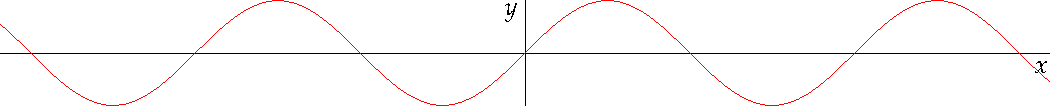
\includegraphics[width=\linewidth]{fg-tufte-wide-sine}%
  \caption[Example file fg-tufte-wide-sine.tex][2ex]
  {This graph shows $y = \sin x$ from about $x = [-10, 10]$.
  \emph{Notice that this figure takes up the full page width.}}%
  \label{fg-tufte-wide-sine}%
\end{figure*}


\vspace*{1ex} %% required to keep distance from full-width figure above.
\begin{algorithm-wide}[h]{1.55\textwidth}%  1.55\textwith expands to full width of figure above!!
\begin{algorithmic}[1]
\PROCEDURE{\CALL{newPivot.saw}{${\underline \varsigma}_{\omega_{s} -1},Walk_{\omega_{s} -1}$}}
\STATE $\mathbb{Z} \gets i = 1,2, \ldots ,L $ 
\STATE $\mathbb{Z}_p \gets permute(\mathbb{Z}) $ 
\STATE ${\cal N} ({\underline \varsigma}_{\omega_{s} -1}) \gets  \{{\underline \varsigma}_{\omega_{s} -1}^i | d({\underline \varsigma}_{\omega_{s} -1}, {\underline \varsigma}_{\omega_{s} -1}^i ) = 1, i \in \mathbb{Z}_p\}$ 
\STATE ${\cal N}_{saw} ({\underline \varsigma}_{\omega_{s} -1}) \gets  \{ {\cal N} ({\underline \varsigma}_{\omega -1}) |
                      {\underline \varsigma}_{\omega_{s} -1}^i \not\in  Walk_{\omega_{s} -1}\}$
   \IF {\strut  ${\cal N}_{saw}  ({\underline \varsigma}_{\omega_{s} -1}) \not= \emptyset$}  
        \STATE ${\underline \varsigma}_{\omega_{s}}\!:\!\Theta({\underline \varsigma}_{\omega_{s}}) \gets {\tt bestNeighbor}({\cal N}_{saw} ({\underline \varsigma}_{\omega_{s} -1}))$
        \STATE $Walk_{\omega_{s}} \gets Walk_{\omega_{s}-1} \cup \{{\underline \varsigma}_{\omega_{s}}\}$
        \STATE $\tau \gets \tau + |~{\cal N}_{saw} ({\underline \varsigma}_{\omega_{s} -1})~| $ 
        \COMMENT{update $cntProbe$}
   \ELSE[\textbf{deal with a trapped pivot}]
        \STATE $\beta = \beta + 1$ 
        \STATE ${\underline \varsigma}_{\omega_{s}}\!:\!\Theta({\underline \varsigma}_{\omega_{s}}) \gets {\tt coordInit}()$ 
        \COMMENT{re-initialize}
        \STATE $Walk_{\omega_{s}} \gets \{ {\underline \varsigma}_{\omega_{s}} \}$
        \STATE $\tau \gets \tau + 1 $ 
        \COMMENT{update $cntProbe$}
    \ENDIF
\STATE \textbf{return} $Walk_{\omega_{s}}\!:\!{\underline \varsigma}_{\omega_{s}}\!:\!\Theta({\underline \varsigma}_{\omega_{s}})$ 
\ENDPROCEDURE 
\end{algorithmic}
\caption[Algorithm file: alg-newPivot-wide.tex]{Procedure newPivot.saw -- using algorithm-wide environment.} 
\label{alg-newPivot-wide}
\end{algorithm-wide}

\newthought{Notably}, typesetting of the Algorithm~\ref{alg-newPivot-wide} results in excessive width, for better rendition 
of identical algorithm, see
Algorithm~\ref{alg-newPivot-normal} in the preceding page.

\lipsum[4]

\newthought{On the next page}, Algorithm~\ref{alg-global-search2-normal}
takes a full page at normal width. However, the version
in  Algorithm~\ref{alg-global-search2-wide} describes the same
algorithm, also on a full page, but in a wider, easier-to-read 
format.


\begin{algorithm}[!T]
\begin{footnotesize}
\begin{minipage}[!T]{0.99\linewidth}
\begin{algorithmic}[1]
\PROCEDURE{\CALL{lssOrel}{$\sigma_0, \Theta^{ub}_L, t_{lmt}, \omega_{lmt}$}}
\STATE {${\underline \varsigma}_0\!:\!\Theta({\underline \varsigma}_0) \gets {\tt coordInit}(\sigma_0)$}
\COMMENT{initial solution}
\STATE $\tau \gets 1 $ 
\COMMENT {initialize cntProbe}
\STATE ${\underline \varsigma^*}\!:\!\Theta({\underline \varsigma^*}) \gets {\underline \varsigma}_0\!:\!\Theta({\underline \varsigma}_0)$ 
\COMMENT{initial best solution} 
\STATE $isCens \gets 0$
\COMMENT{initialize $isCensored$}
\STATE $tgReached \gets 0$                                     
\COMMENT{initialize $targetReached$}
\STATE $\beta \gets 0$                                         
\COMMENT{initialize $cntTrapped$}
\STATE $\omega \gets 0$                                        
\COMMENT{initialize total number of steps}
\WHILE {{\bf true}}
  \STATE $\omega_{s}\!:\!{\underline \varsigma^*}\!:\!\Theta({\underline \varsigma^*}) \gets {\tt walk.saw}({\underline \varsigma}_{0}\!:\!\Theta({\underline \varsigma}_{0}),t_{lmt},\omega_{lmt})$ 
  \COMMENT{return a completed walk segment}
  \STATE $\omega \gets \omega + \omega_{s} $                   
  \COMMENT{update total number of steps}
  \IF{$\Theta({\underline \varsigma^*}) \leq \Theta^{ub}_L$}
    \IF {$\Theta({\underline \varsigma^*}) = \Theta^{ub}_L$}
      \STATE{$tgReached = 1$}                                  
      \COMMENT{upper-bound is reached}
    \ELSE
      \STATE $tgReached = 2$                                   
      \COMMENT{upper-bound is improved}
    \ENDIF
    \STATE {\bf{break}}
  \ENDIF
  \IF{$t \geq t_{lmt}$}
    \STATE $isCens \gets 1$                                    
    \COMMENT{return solution as ``censored''}
    \STATE {\bf{break}}
  \ENDIF
  \STATE ${\underline \varsigma}_0\!:\!\Theta({\underline \varsigma}_0) \gets {\tt coordInit}()$ 
  \COMMENT{initialize a new walk segment}
  \STATE $\tau \gets \tau + 1 $                               
  \COMMENT{update $cntProbe$}
  \STATE $\omega \gets \omega + 1 $                           
  \COMMENT{update total number of steps}
\ENDWHILE
\STATE $Table \gets (\sigma_0, {\underline \varsigma^*}, \Theta({\underline \varsigma^*}), \omega, \tau, t, isCens, tgReached)$
\ENDPROCEDURE
\end{algorithmic}
\end{minipage}

\vspace{0.2cm}
\begin{minipage}[!T]{0.49\linewidth}
\begin{algorithmic}[1]
\PROCEDURE{\CALL{walk.saw}{${\underline \varsigma}_{0}\!:\!\Theta({\underline \varsigma}_{0}),t_{lmt}, \omega_{lmt}$}}
\IF {$\Theta({\underline \varsigma}_{0}) \le \Theta({\underline \varsigma^*})$}
    \STATE ${\underline \varsigma^*}\!:\!\Theta({\underline \varsigma^*}) \gets {\underline \varsigma}_0\!:\!\Theta({\underline \varsigma}_0)$
    \COMMENT{new best solution}
\ENDIF
\STATE $\omega_{s} \gets 0$     
\COMMENT{walk segment length}                                   
\STATE $Walk_{0} \gets \{ {\underline \varsigma}_0 \}$
\COMMENT{new walk segment}
\WHILE {$\Theta({\underline \varsigma^*})  > \Theta^{ub}_L$ \textbf{and} $\omega_{s} < \omega_{lmt}$}
    \IF [timeout]{$t \geq t_{lmt}$}
        \STATE {\bf break}
    \ENDIF
    \STATE $\omega_{s}=\omega_{s}+1$
    \COMMENT{{\bf a new step!}}
    \STATE $Walk_{\omega_{s}}\!:\!{\underline \varsigma}_{\omega_{s}}\!:\!\Theta({\underline \varsigma}_{\omega_{s}}) \gets$
    \STATE { \hspace{0.5cm} $ \gets {\tt newPivot.saw}({\underline \varsigma}_{\omega_{s} - 1}, Walk_{\omega_{s} - 1})$}
     \IF { $\Theta({\underline \varsigma}_{\omega_{s}}) \le \Theta({\underline \varsigma^*})$} 
       \STATE ${\underline \varsigma^*}\!:\!\Theta({\underline \varsigma^*}) \gets {\underline \varsigma_{\omega_{s}}}\!:\!\Theta({\underline \varsigma}_{\omega_{s}})$
     \ENDIF
\ENDWHILE
\STATE {\bf return} $\omega_{s}\!:\!{\underline \varsigma^*}\!:\!\Theta({\underline \varsigma^*})$
\ENDPROCEDURE
\end{algorithmic}
\end{minipage}
\begin{minipage}[!T]{0.49\linewidth}
\label{fg_global_search_c}
\begin{algorithmic}[1]
\PROCEDURE{\CALL{newPivot.saw}{${\underline \varsigma}_{\omega_{s} -1},Walk_{\omega_{s} -1}$}}
\STATE $\mathbb{Z} \gets i = 1,2, \ldots ,L $ 
\STATE $\mathbb{Z}_p \gets permute(\mathbb{Z}) $ 
\STATE ${\cal N} ({\underline \varsigma}_{\omega_{s} -1}) \gets  \{{\underline \varsigma}_{\omega_{s} -1}^i | d({\underline \varsigma}_{\omega_{s} -1}, {\underline \varsigma}_{\omega_{s} -1}^i ) = 1, i \in \mathbb{Z}_p\}$ 
\STATE ${\cal N}_{saw} ({\underline \varsigma}_{\omega_{s} -1}) \gets  \{ {\cal N} ({\underline \varsigma}_{\omega -1}) |
                      {\underline \varsigma}_{\omega_{s} -1}^i \not\in  Walk_{\omega_{s} -1}\}$
   \IF {\strut  ${\cal N}_{saw}  ({\underline \varsigma}_{\omega_{s} -1}) \not= \emptyset$}  
        \STATE ${\underline \varsigma}_{\omega_{s}}\!:\!\Theta({\underline \varsigma}_{\omega_{s}}) \gets {\tt bestNeighbor}({\cal N}_{saw} ({\underline \varsigma}_{\omega_{s} -1}))$
        \STATE $Walk_{\omega_{s}} \gets Walk_{\omega_{s}-1} \cup \{{\underline \varsigma}_{\omega_{s}}\}$
        \STATE $\tau \gets \tau + |~{\cal N}_{saw} ({\underline \varsigma}_{\omega_{s} -1})~| $ 
        \COMMENT{update $cntProbe$}
   \ELSE[\textbf{deal with a trapped pivot}]
        \STATE $\beta = \beta + 1$ 
        \STATE ${\underline \varsigma}_{\omega_{s}}\!:\!\Theta({\underline \varsigma}_{\omega_{s}}) \gets {\tt coordInit}()$ 
        \COMMENT{re-initialize}
        \STATE $Walk_{\omega_{s}} \gets \{ {\underline \varsigma}_{\omega_{s}} \}$
        \STATE $\tau \gets \tau + 1 $ 
        \COMMENT{update $cntProbe$}
    \ENDIF
\STATE \textbf{return} $Walk_{\omega_{s}}\!:\!{\underline \varsigma}_{\omega_{s}}\!:\!\Theta({\underline \varsigma}_{\omega_{s}})$ 
\ENDPROCEDURE 
\end{algorithmic}
\end{minipage}
\caption[Algorithm file: alg-global-search2-normal.tex]{A fully instrumented version of solver \lssOrel\ -- normal width.} 
\label{alg-global-search2-normal}
\end{footnotesize}
\end{algorithm}

%\begin{Algorithm}[!T]{15cm}
\begin{algorithm-wide}[h]{1.5\textwidth}%  1.55\textwith expands to full width of widest figure
\begin{footnotesize}
\begin{minipage}[!T]{0.99\linewidth}
\begin{algorithmic}[1]
\PROCEDURE{\CALL{lssOrel}{$\sigma_0, \Theta^{ub}_L, t_{lmt}, \omega_{lmt}$}}
\STATE {${\underline \varsigma}_0\!:\!\Theta({\underline \varsigma}_0) \gets {\tt coordInit}(\sigma_0)$}
\COMMENT{initial solution}
\STATE $\tau \gets 1 $ 
\COMMENT {initialize cntProbe}
\STATE ${\underline \varsigma^*}\!:\!\Theta({\underline \varsigma^*}) \gets {\underline \varsigma}_0\!:\!\Theta({\underline \varsigma}_0)$ 
\COMMENT{initial best solution} 
\STATE $isCens \gets 0$
\COMMENT{initialize $isCensored$}
\STATE $tgReached \gets 0$                                     
\COMMENT{initialize $targetReached$}
\STATE $\beta \gets 0$                                         
\COMMENT{initialize $cntTrapped$}
\STATE $\omega \gets 0$                                        
\COMMENT{initialize total number of steps}
\WHILE {{\bf true}}
  \STATE $\omega_{s}\!:\!{\underline \varsigma^*}\!:\!\Theta({\underline \varsigma^*}) \gets {\tt walk.saw}({\underline \varsigma}_{0}\!:\!\Theta({\underline \varsigma}_{0}),t_{lmt},\omega_{lmt})$ 
  \COMMENT{return a completed walk segment}
  \STATE $\omega \gets \omega + \omega_{s} $                   
  \COMMENT{update total number of steps}
  \IF{$\Theta({\underline \varsigma^*}) \leq \Theta^{ub}_L$}
    \IF {$\Theta({\underline \varsigma^*}) = \Theta^{ub}_L$}
      \STATE{$tgReached = 1$}                                  
      \COMMENT{upper-bound is reached}
    \ELSE
      \STATE $tgReached = 2$                                   
      \COMMENT{upper-bound is improved}
    \ENDIF
    \STATE {\bf{break}}
  \ENDIF
  \IF{$t \geq t_{lmt}$}
    \STATE $isCens \gets 1$                                    
    \COMMENT{return solution as ``censored''}
    \STATE {\bf{break}}
  \ENDIF
  \STATE ${\underline \varsigma}_0\!:\!\Theta({\underline \varsigma}_0) \gets {\tt coordInit}()$ 
  \COMMENT{initialize a new walk segment}
  \STATE $\tau \gets \tau + 1 $                               
  \COMMENT{update $cntProbe$}
  \STATE $\omega \gets \omega + 1 $                           
  \COMMENT{update total number of steps}
\ENDWHILE
\STATE $Table \gets (\sigma_0, {\underline \varsigma^*}, \Theta({\underline \varsigma^*}), \omega, \tau, t, isCens, tgReached)$
\ENDPROCEDURE
\end{algorithmic}
\end{minipage}

\vspace{0.2cm}
\begin{minipage}[!T]{0.49\linewidth}
\begin{algorithmic}[1]
\PROCEDURE{\CALL{walk.saw}{${\underline \varsigma}_{0}\!:\!\Theta({\underline \varsigma}_{0}),t_{lmt}, \omega_{lmt}$}}
\IF {$\Theta({\underline \varsigma}_{0}) \le \Theta({\underline \varsigma^*})$}
    \STATE ${\underline \varsigma^*}\!:\!\Theta({\underline \varsigma^*}) \gets {\underline \varsigma}_0\!:\!\Theta({\underline \varsigma}_0)$
    \COMMENT{new best solution}
\ENDIF
\STATE $\omega_{s} \gets 0$     
\COMMENT{walk segment length}                                   
\STATE $Walk_{0} \gets \{ {\underline \varsigma}_0 \}$
\COMMENT{new walk segment}
\WHILE {$\Theta({\underline \varsigma^*})  > \Theta^{ub}_L$ \textbf{and} $\omega_{s} < \omega_{lmt}$}
    \IF [timeout]{$t \geq t_{lmt}$}
        \STATE {\bf break}
    \ENDIF
    \STATE $\omega_{s}=\omega_{s}+1$
    \COMMENT{{\bf a new step!}}
    \STATE $Walk_{\omega_{s}}\!:\!{\underline \varsigma}_{\omega_{s}}\!:\!\Theta({\underline \varsigma}_{\omega_{s}}) \gets$
    \STATE { \hspace{0.5cm} $ \gets {\tt newPivot.saw}({\underline \varsigma}_{\omega_{s} - 1}, Walk_{\omega_{s} - 1})$}
     \IF { $\Theta({\underline \varsigma}_{\omega_{s}}) \le \Theta({\underline \varsigma^*})$} 
       \STATE ${\underline \varsigma^*}\!:\!\Theta({\underline \varsigma^*}) \gets {\underline \varsigma_{\omega_{s}}}\!:\!\Theta({\underline \varsigma}_{\omega_{s}})$
     \ENDIF
\ENDWHILE
\STATE {\bf return} $\omega_{s}\!:\!{\underline \varsigma^*}\!:\!\Theta({\underline \varsigma^*})$
\ENDPROCEDURE
\end{algorithmic}
\end{minipage}
\begin{minipage}[!T]{0.49\linewidth}
\label{alg-global-search2-wide-c}
\begin{algorithmic}[1]
\PROCEDURE{\CALL{newPivot.saw}{${\underline \varsigma}_{\omega_{s} -1},Walk_{\omega_{s} -1}$}}
\STATE $\mathbb{Z} \gets i = 1,2, \ldots ,L $ 
\STATE $\mathbb{Z}_p \gets permute(\mathbb{Z}) $ 
\STATE ${\cal N} ({\underline \varsigma}_{\omega_{s} -1}) \gets  \{{\underline \varsigma}_{\omega_{s} -1}^i | d({\underline \varsigma}_{\omega_{s} -1}, {\underline \varsigma}_{\omega_{s} -1}^i ) = 1, i \in \mathbb{Z}_p\}$ 
\STATE ${\cal N}_{saw} ({\underline \varsigma}_{\omega_{s} -1}) \gets  \{ {\cal N} ({\underline \varsigma}_{\omega -1}) |
                      {\underline \varsigma}_{\omega_{s} -1}^i \not\in  Walk_{\omega_{s} -1}\}$
   \IF {\strut  ${\cal N}_{saw}  ({\underline \varsigma}_{\omega_{s} -1}) \not= \emptyset$}  
        \STATE ${\underline \varsigma}_{\omega_{s}}\!:\!\Theta({\underline \varsigma}_{\omega_{s}}) \gets {\tt bestNeighbor}({\cal N}_{saw} ({\underline \varsigma}_{\omega_{s} -1}))$
        \STATE $Walk_{\omega_{s}} \gets Walk_{\omega_{s}-1} \cup \{{\underline \varsigma}_{\omega_{s}}\}$
        \STATE $\tau \gets \tau + |~{\cal N}_{saw} ({\underline \varsigma}_{\omega_{s} -1})~| $ 
        \COMMENT{update $cntProbe$}
   \ELSE[\textbf{deal with a trapped pivot}]
        \STATE $\beta = \beta + 1$ 
        \STATE ${\underline \varsigma}_{\omega_{s}}\!:\!\Theta({\underline \varsigma}_{\omega_{s}}) \gets {\tt coordInit}()$ 
        \COMMENT{re-initialize}
        \STATE $Walk_{\omega_{s}} \gets \{ {\underline \varsigma}_{\omega_{s}} \}$
        \STATE $\tau \gets \tau + 1 $ 
        \COMMENT{update $cntProbe$}
    \ENDIF
\STATE \textbf{return} $Walk_{\omega_{s}}\!:\!{\underline \varsigma}_{\omega_{s}}\!:\!\Theta({\underline \varsigma}_{\omega_{s}})$ 
\ENDPROCEDURE 
\end{algorithmic}
\end{minipage}
\caption[Algorithm file: alg-global-search2-wide.tex]{A fully instrumented version of solver \lssOrel\ -- using algorithm-wide environment.} 
\label{alg-global-search2-wide}
\end{footnotesize}
\end{algorithm-wide}

\clearpage
%\begin{algorithm-wide}[h]{15cm}
\begin{algorithm-wide}[!t]{1.5\textwidth}%  1.55\textwith expands to full width of widest figure
\begin{footnotesize}
\begin{minipage}[!T]{0.52\linewidth}
\centering
\begin{algorithmic}[1]
\PROCEDURE{\CALL{lssMAts}{$\Theta^{ub}_L, t_{lmt}$}}
\FOR{$i\gets 1$ {\bf to} $popsize$} \label{alg_lssMAts_For1}
    \STATE $pop_i\gets$ \CALL{RandomBinarySequence}{$L$}
    \STATE \CALL{Evaluate}{$pop_i$}
\ENDFOR \label{alg_lssMAts_For2}
\STATE \colorbox{Gray}{\valueBest $\gets \CALL{ValueBest}{pop}$}
\WHILE {\colorbox{Gray}{ $t < t_{lmt}$ {\bf ~and~}  \valueBest $\,>\,$ \valueTarget} }
    \FOR{$i=1$ {\bf to} $\mathit{offsize}$}     
        \IF {recombination is performed ($p_X$)} \label{alg_lssMAts_Rec1}
            \STATE $parent_1 \gets $\CALL{Select}{$pop$}
            \STATE $parent_2 \gets $\CALL{Select}{$pop$}
            \STATE $\mathit{offspring_i}\gets$\CALL{Recombine}{$parent_1, parent_2$}
        \ELSE
            \STATE $\mathit{offspring}_i \gets $\CALL{Select}{$pop$}
        \ENDIF \label{alg_lssMAts_Rec2}
        \IF {mutation is performed ($p_m$)} \label{alg_lssMAts_Mut1}
            \STATE $\mathit{offspring}_i \gets $\CALL{Mutate}{$\mathit{offspring}_i$}
        \ENDIF \label{alg_lssMAts_Mut2}
        \STATE $\mathit{offspring}_i \gets$\CALL{TabuSearch}{$\mathit{offspring}_i$}
        \STATE \CALL{Evaluate}{$\mathit{offspring}_i$}
    \ENDFOR
    \STATE $pop \gets$\CALL{Replace}{$pop$, $\mathit{offspring}$} \label{alg_lssMAts_Sel}
    \STATE \colorbox{Gray}{\valueBest $\gets \CALL{ValueBest}{pop}$}
\ENDWHILE
\ENDPROCEDURE 
\end{algorithmic}
\end{minipage}
\begin{minipage}[!T]{0.52\linewidth}
% {\small	
% % The procedure \lssMAts\ on the left is an instrumented versions of the 
% % \labs\ solver named as $MA_{TS}$
% % in~\cite{Lib-OPUS-labs-2009-ASC-Gallardo-memetic}.
% % Settings of all parameters,
% % used also in our experiments, are described
% % in~\cite{Lib-OPUS-labs-2009-ASC-Gallardo-memetic}.
% % See a concise reprise below.
\par\vspace*{1ex}
\begin{tabular}{l l}
 {\bf setting} & {\bf value} \\
 \hline
 population size: & 100 \\
 mutation probability: & $2/(L+1)$ \\
 crossover probability: & 0.9 \\
 tournament selection size: & 2 \\
 crossover: & uniform \\
 tabu search walk length: & a random choice  \\
 ~~              &  from the range\\
 ~~              & {\small [$\frac{L}{2}, \frac{3 L}{2}$]}\\
 ~~              & ~~
\end{tabular}
%\centering
\begin{algorithmic}[1]
\PROCEDURE{\CALL{lssRRts}{$\Theta^{ub}_L, t_{lmt}$}}
\STATE $pop_1\gets$ \CALL{RandomBinarySequence}{$L$}
\STATE \CALL{Evaluate}{$pop_1$}
\STATE \colorbox{Gray} {\valueBest $\gets \CALL{ValueBest}{pop}$}
\WHILE {\colorbox{Gray}{ $t < t_{lmt}$ {\bf ~and~}  \valueBest $\,>\,$ \valueTarget} }
        \STATE $\mathit{pop_1} \gets $\CALL{RandomBinarySequence}{$L$}
        \STATE $\mathit{pop_1} \gets $\CALL{TabuSearch}{$\mathit{pop_1}$}
        \STATE \CALL{Evaluate}{$\mathit{pop_1}$}
        \STATE \colorbox{Gray}{\valueBest $\gets \CALL{ValueBest}{pop}$}
\ENDWHILE
\ENDPROCEDURE 
\end{algorithmic}
\vspace{2cm}
\end{minipage}
\caption[Algorithm file: alg-lssMAts-lssRRts-wide.tex]{\lssMAts\ and \lssRRts\ algorithms -- using algorithm-wide environment.} 
\label{alg-lssMAts-lssRRts-wide}
\end{footnotesize}
\end{algorithm-wide}

\newthought{On this page}, Algorithm~\ref{alg-lssMAts-lssRRts-wide}
is placed at the top of the page with the [!t] option.
\lipsum[4]
\lipsum[1]

\newthought{Here is} a simple in-line Algorithm description we can include, with some restrictions, in a margin note as well.
\begin{algorithm}
\begin{algorithmic}[1]
\PROCEDURE{\CALL{lssRRts}{$\Theta^{ub}_L, t_{lmt}$}}
\STATE $pop_1\gets$ \CALL{RandomBinarySequence}{$L$}
\STATE \CALL{Evaluate}{$pop_1$}
\STATE \colorbox{Gray} {\valueBest $\gets \CALL{ValueBest}{pop}$}
\WHILE {\colorbox{Gray}{ $t < t_{lmt}$ {\bf ~and~}  \valueBest $\,>\,$ \valueTarget} }
        \STATE $\mathit{pop_1} \gets $\CALL{RandomBinarySequence}{$L$}
        \STATE $\mathit{pop_1} \gets $\CALL{TabuSearch}{$\mathit{pop_1}$}
        \STATE \CALL{Evaluate}{$\mathit{pop_1}$}
        \STATE \colorbox{Gray}{\valueBest $\gets \CALL{ValueBest}{pop}$}
\ENDWHILE
\ENDPROCEDURE 
\end{algorithmic}
\caption{Pseudo code for \lssRRts\ -- in-line version}.
\end{algorithm}

\newthought{Here is a margin note} for a 
pseudo-code that describes a simple procedure\marginnote[-6ex]{
%\begin{algorithm} %%%% does NOT work with \marginnote
\begin{algorithmic}[1]
\PROCEDURE{\CALL{lssRRts}{$\Theta^{ub}_L, t_{lmt}$}}
\STATE $pop_1\gets$ \CALL{RandBinSeq}{$L$}
\STATE \CALL{Evaluate}{$pop_1$}
\STATE \colorbox{Gray} {\valueBest $\gets \CALL{ValueBest}{pop}$}
\WHILE {\colorbox{Gray}{ $t < t_{lmt}$ {\bf ~and~}  \valueBest $\,>\,$ \valueTarget} }
        \STATE $\mathit{pop_1} \gets $\CALL{RandBinSeq}{$L$}
        \STATE $\mathit{pop_1} \gets $\CALL{TabuSearch}{$\mathit{pop_1}$}
        \STATE \CALL{Evaluate}{$\mathit{pop_1}$}
        \STATE \colorbox{Gray}{\valueBest $\gets \CALL{ValueBest}{pop}$}
\ENDWHILE
\ENDPROCEDURE 
\end{algorithmic}
%\caption{Pseudo code for \lssRRts}.
%\end{algorithm}
}. NOTE: we cannot use the \verb+\algorithm+ and \verb+\caption+ environment 
under  \verb+\marginnote+.

\lipsum[4]


 

\chapter{About Figures}
\label{chap-Figures}
\newthought{Figures in this chapter} are divided into two sections: 
(1) figures from Tufte,
(2) figures from other sources.

\newthought{For details} about how various text items are being represented,
see Chapter~\ref{chap-About}.

%\chapter{About Figures}
%\label{chap-AboutFigures}
%\newthought{Figures in this chapter} are divided into two sections: 
%(1) figures from Tufte,
%(2) figures from other sources.
%
\section{Figures from Tufte}
\label{chap-Figures-Tufte}

\newthought{About the figures}  from Tufte:
\begin{itemize}
\item
a margin figure, {\tt fg-tufte-margin-helix}, Figure~\ref{fg-tufte-margin-helix}, 
\item
a normal-width figure, {\tt fg-tufte-normal-hilbertcurves}, Figure~\ref{fg-tufte-normal-hilbertcurves}, and
\item
a full-width figure, {\tt fg-tufte-wide-sine}, Figure~\ref{fg-tufte-wide-sine}.
\end{itemize}


\begin{marginfigure}[-50ex]%
  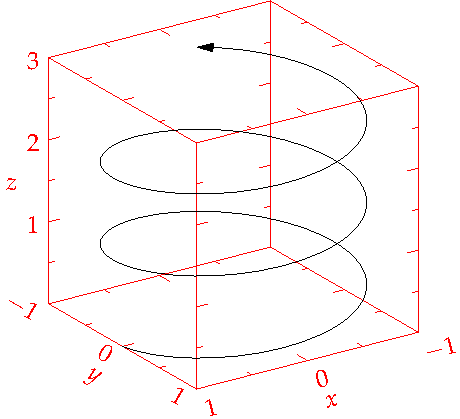
\includegraphics[width=\linewidth]{fg-tufte-margin-helix}
  \caption[Example file fg-tufte-margin-helix.tex]
  {This is a margin figure.  
    The helix is defined by 
    $x = \cos(2\pi z)$, $y = \sin(2\pi z)$, and $z = [0, 2.7]$. The figure was
    drawn using Asymptote (\url{http://asymptote.sf.net/}).}
  \label{fg-tufte-margin-helix}
\end{marginfigure}.






\begin{figure}[h!]%
  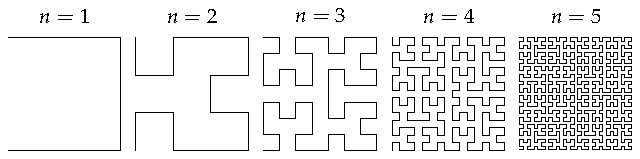
\includegraphics{fg-tufte-normal-hilbertcurves}
  \caption[Example file fg-tufte-normal-hilbertcurves.tex][6ex]
  {Hilbert curves of various degrees $n$. 
  \emph{Notice that this figure only takes up the main textblock width.}}
  \label{fg-tufte-normal-hilbertcurves}
\end{figure}

\lipsum[2]
\begin{figure*}[t!]
  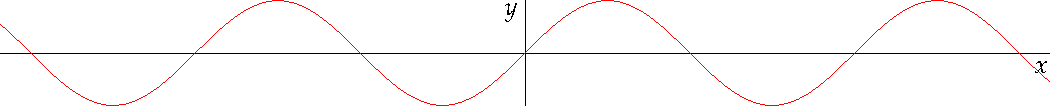
\includegraphics[width=\linewidth]{fg-tufte-wide-sine}%
  \caption[Example file fg-tufte-wide-sine.tex][2ex]
  {This graph shows $y = \sin x$ from about $x = [-10, 10]$.
  \emph{Notice that this figure takes up the full page width.}}%
  \label{fg-tufte-wide-sine}%
\end{figure*}
%\chapter{About Figures}
%\label{chap-AboutFigures}
%\newthought{Figures in this chapter} are divided into two sections: 
%(1) figures from Tufte,
%(2) figures from other sources.
%

\section{Figures from Other Sources}
\label{chap-AboutFigures-Other}

\newthought{The file} {\tt fg-R-labs-wide-4-figures.tex}  
renders Figure~\ref{fg-R-labs-wide-4-figures}, used 
in\cite[27ex]{Lib-OPUS2-labs-2015-arxiv-Boskovic}.
\lipsum[1]
\begin{figure*}[t!]\index{Figures in R!4 panes}
% http://en.wikibooks.org/wiki/LaTeX/Floats,_Figures_and_Captions
% http://tex.stackexchange.com/questions/119984/subfigures-side-by-side-with-captions
%\usepackage{caption}     %% loads OK, but not needed neither subfigure nor subcaption
                          %% work under Tufte-book template
%\usepackage{subfigure}   %% This package loads without errors, however 
                          %% \begin{subfigure}[t]{0.49\textwidth} DOES NOT WORK!
%\usepackage{subcaption}  %% ! Package caption Error: The `subcaption' package does not work 
                          %%   correctly in compatibility mode.
\centering
\vspace*{-5ex}% removes white space at the top

\begin{minipage}{0.49\textwidth}
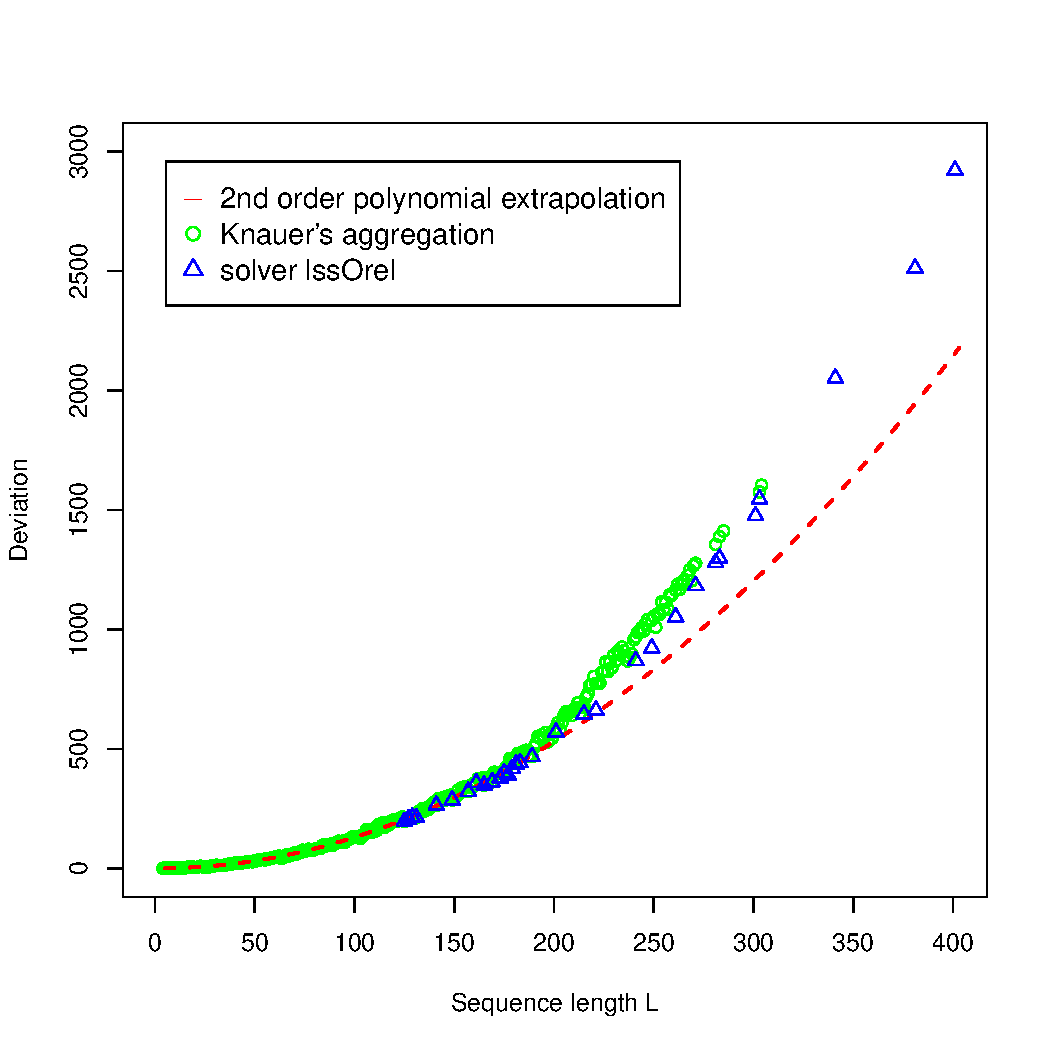
\includegraphics[width=0.99\textwidth]{fg-R-labs-wide-4-figures-a}
\vspace*{-5ex}% removes white space for the next row of figures
\end{minipage}
\begin{minipage}{0.49\textwidth}
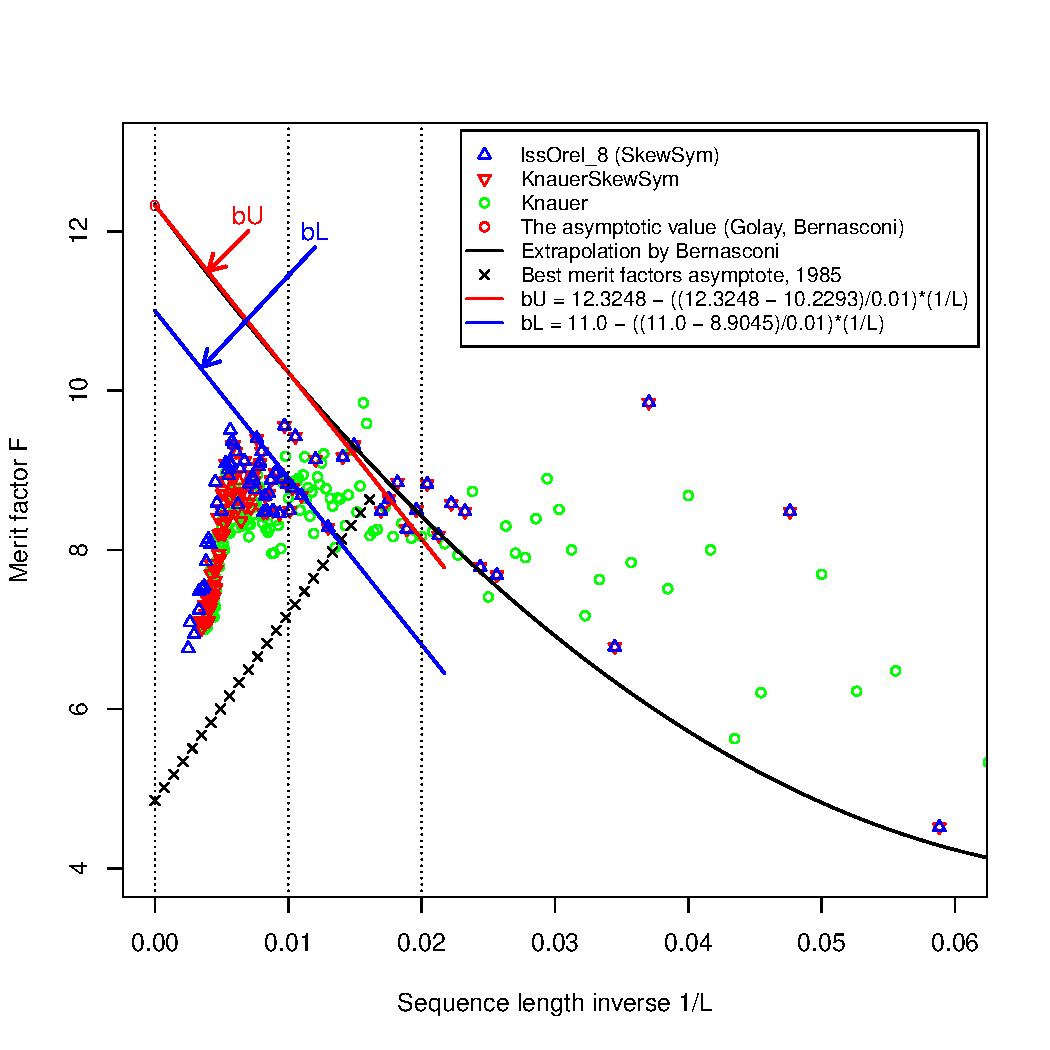
\includegraphics[width=0.99\textwidth]{fg-R-labs-wide-4-figures-b}
\vspace*{-5ex}% removes white space for the next row of figures
\end{minipage}
~%
\begin{minipage}{0.49\textwidth}
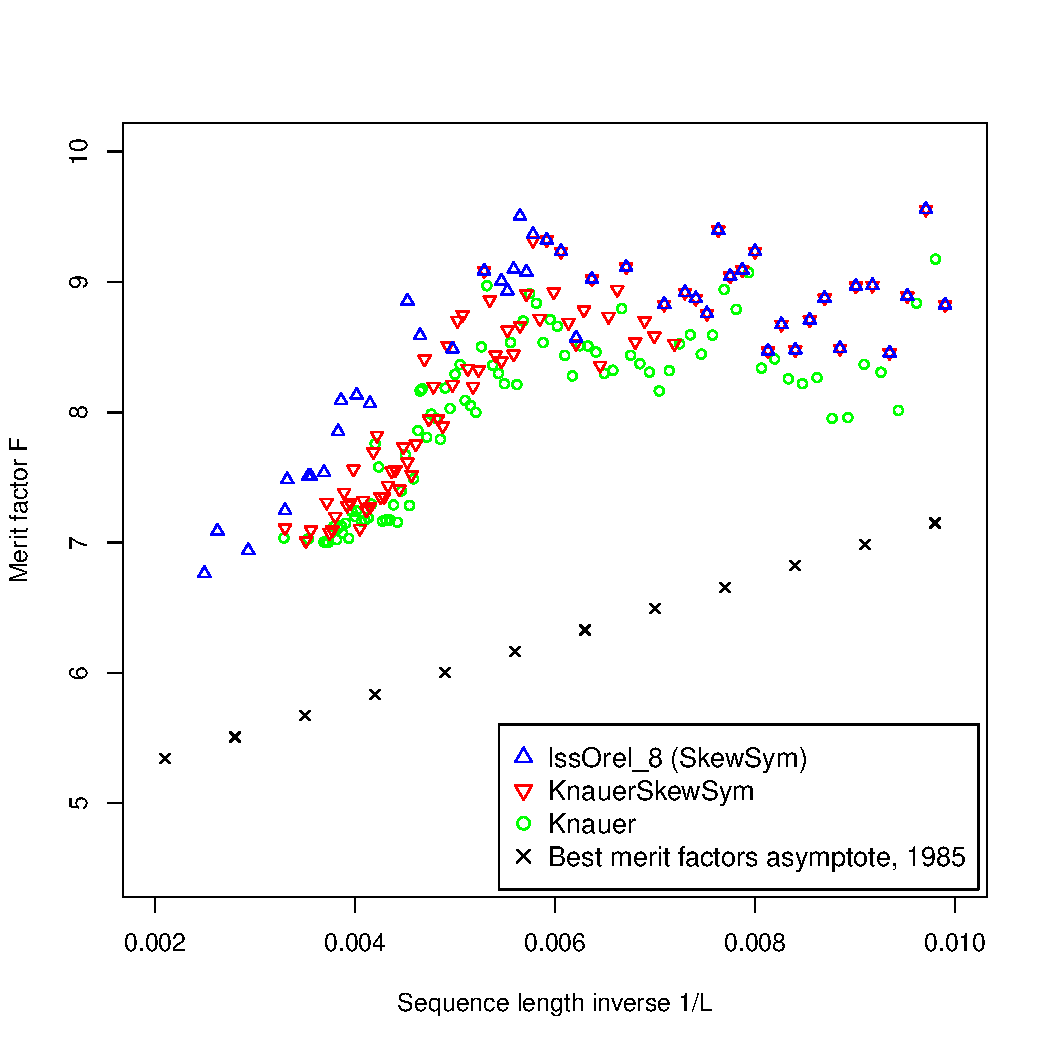
\includegraphics[width=0.99\textwidth]{fg-R-labs-wide-4-figures-c}
%\vspace*{-1ex}
\end{minipage}
%
\begin{minipage}{0.49\textwidth}
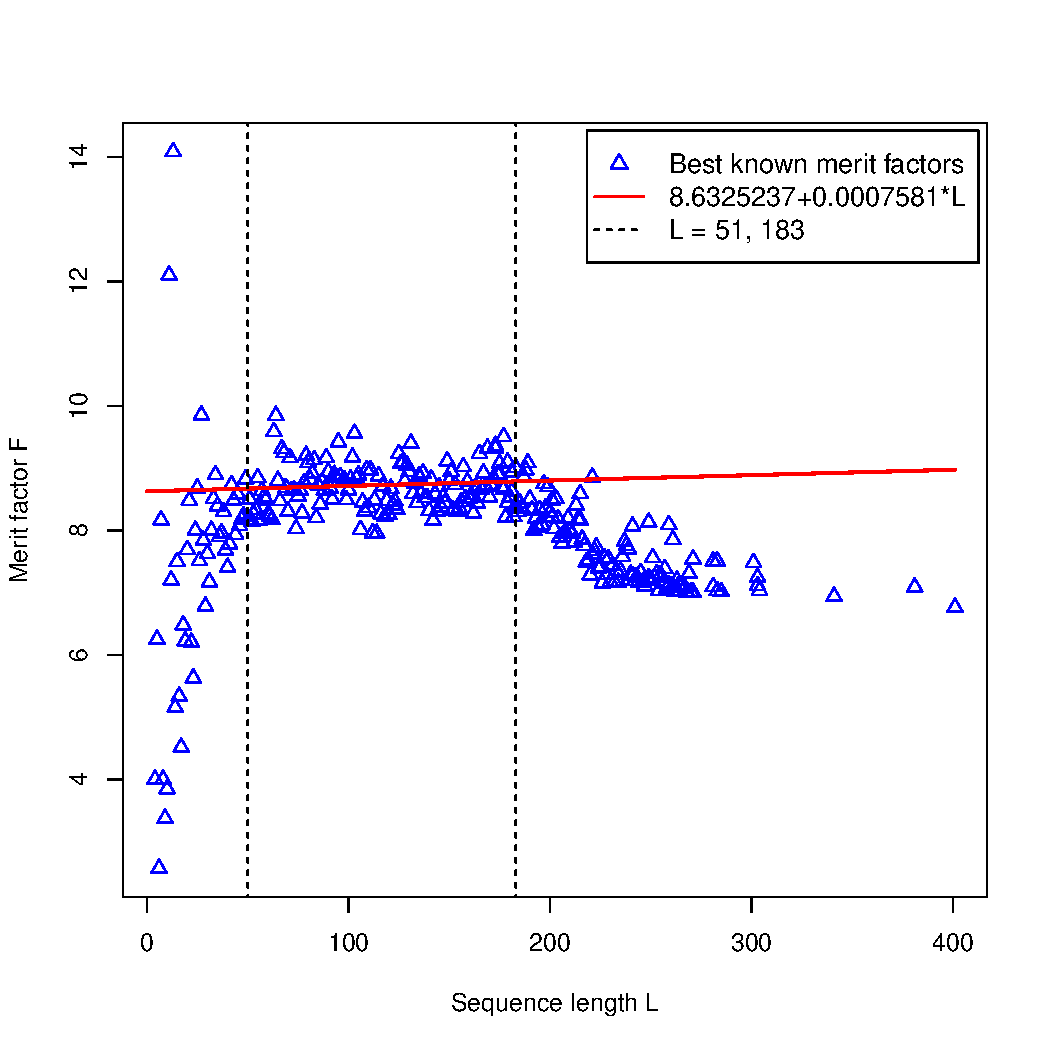
\includegraphics[width=0.99\textwidth]{fg-R-labs-wide-4-figures-d}
%\vspace*{-1ex}
\end{minipage}
%
\caption[From the file fg-R-labs-wide-4-figures.tex][3ex]
{From the file fg-R-labs-wide-4-figures.tex {\em borrowed from} {\tt Lib-OPUS2-labs-2015-arxiv-Boskovic}. 
{\bf NOTE: both `verb' and `cite' commands seem disabled under `figure environment'!}
(a) 
it may not be possible to create (a) in this file with \LaTeX ... may need to create it in R;
%
(b)
it may not be possible to create (b) in this file with \LaTeX ... may need to create it in R;
%
(c)
it may not be possible to create (c) in this file with \LaTeX ... may need to create it in R;
%
(d) 
it may not be possible to create (d) in this file with \LaTeX ... may need to create it in R.
}
\label{fg-R-labs-wide-4-figures}
\end{figure*}



\begin{figure*}[t!]\index{Figures in R!6 panes}
% http://en.wikibooks.org/wiki/LaTeX/Floats,_Figures_and_Captions
% http://tex.stackexchange.com/questions/119984/subfigures-side-by-side-with-captions
%\usepackage{caption}     %% loads OK, but not needed neither subfigure nor subcaption
                          %% work under Tufte-book template
%\usepackage{subfigure}   %% This package loads without errors, however 
                          %% \begin{subfigure}[t]{0.49\textwidth} DOES NOT WORK!
%\usepackage{subcaption}  %% ! Package caption Error: The `subcaption' package does not work 
                          %%   correctly in compatibility mode.
\centering
\vspace*{-5ex}% removes white space at the top

\begin{minipage}{0.49\textwidth}
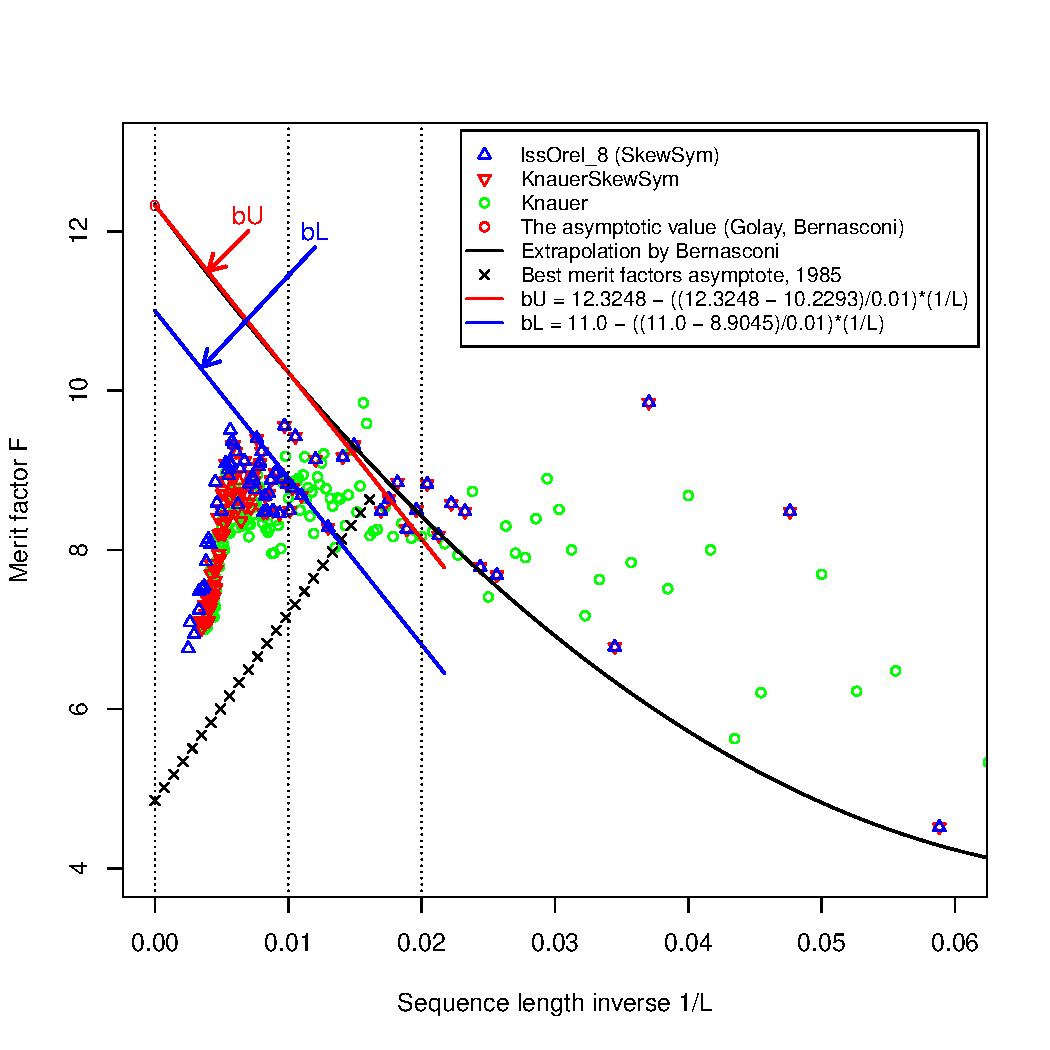
\includegraphics[width=0.99\textwidth]{fg-R-labs-wide-4-figures-b}
\vspace*{-5ex}% removes white space for the next row of figures
\end{minipage}
\begin{minipage}{0.49\textwidth}
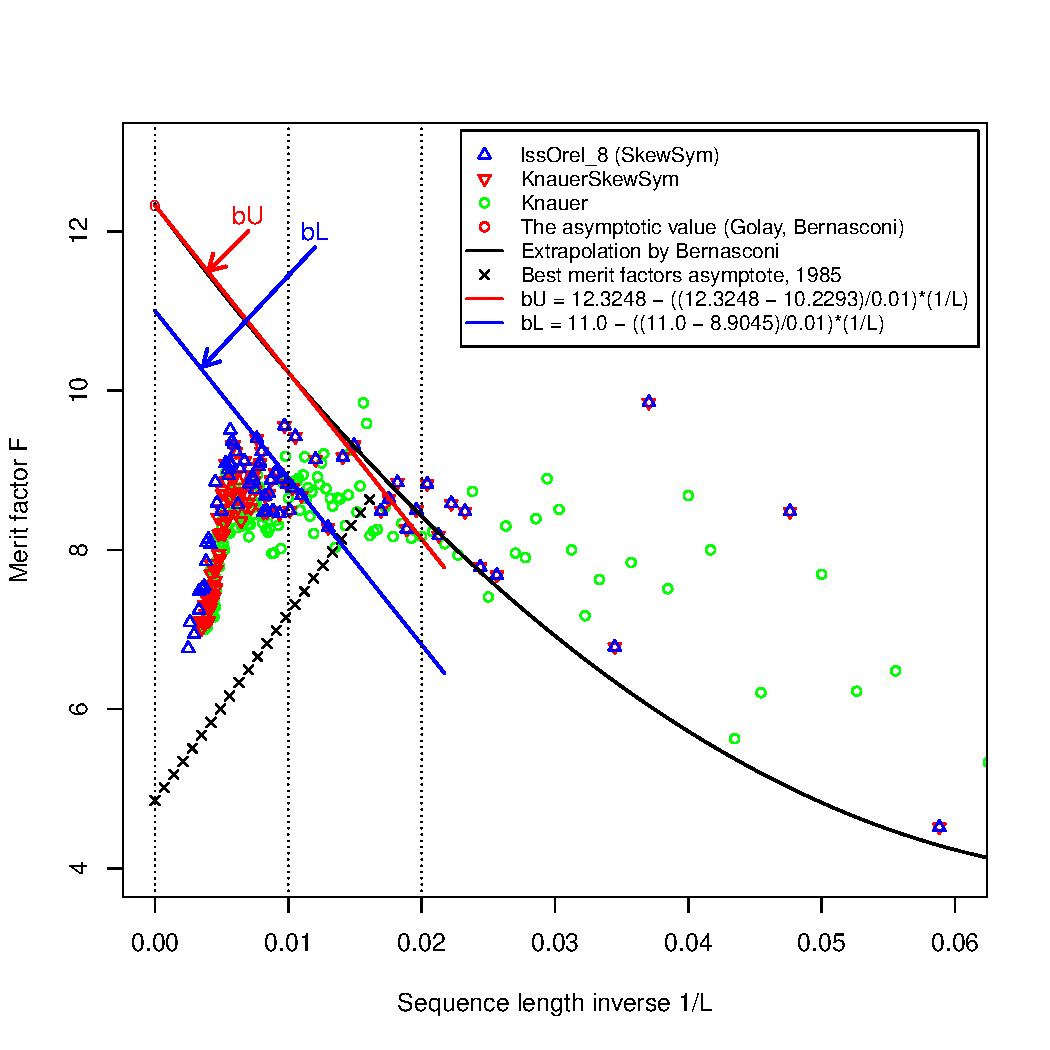
\includegraphics[width=0.99\textwidth]{fg-R-labs-wide-4-figures-b}
\vspace*{-5ex}% removes white space for the next row of figures
\end{minipage}
~%
\begin{minipage}{0.49\textwidth}
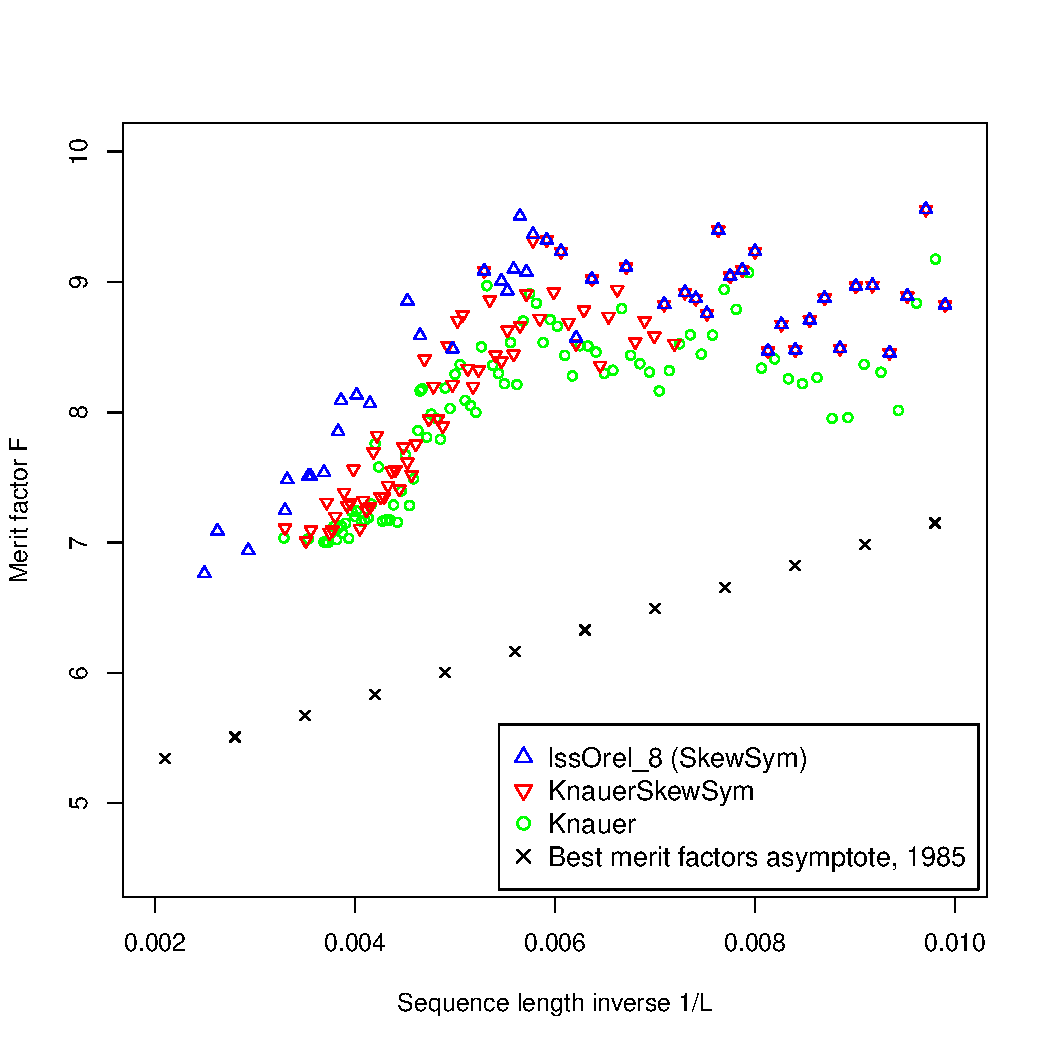
\includegraphics[width=0.99\textwidth]{fg-R-labs-wide-4-figures-c}
\vspace*{-5ex}% removes white space for the next row of figures
\end{minipage}
%
\begin{minipage}{0.49\textwidth}
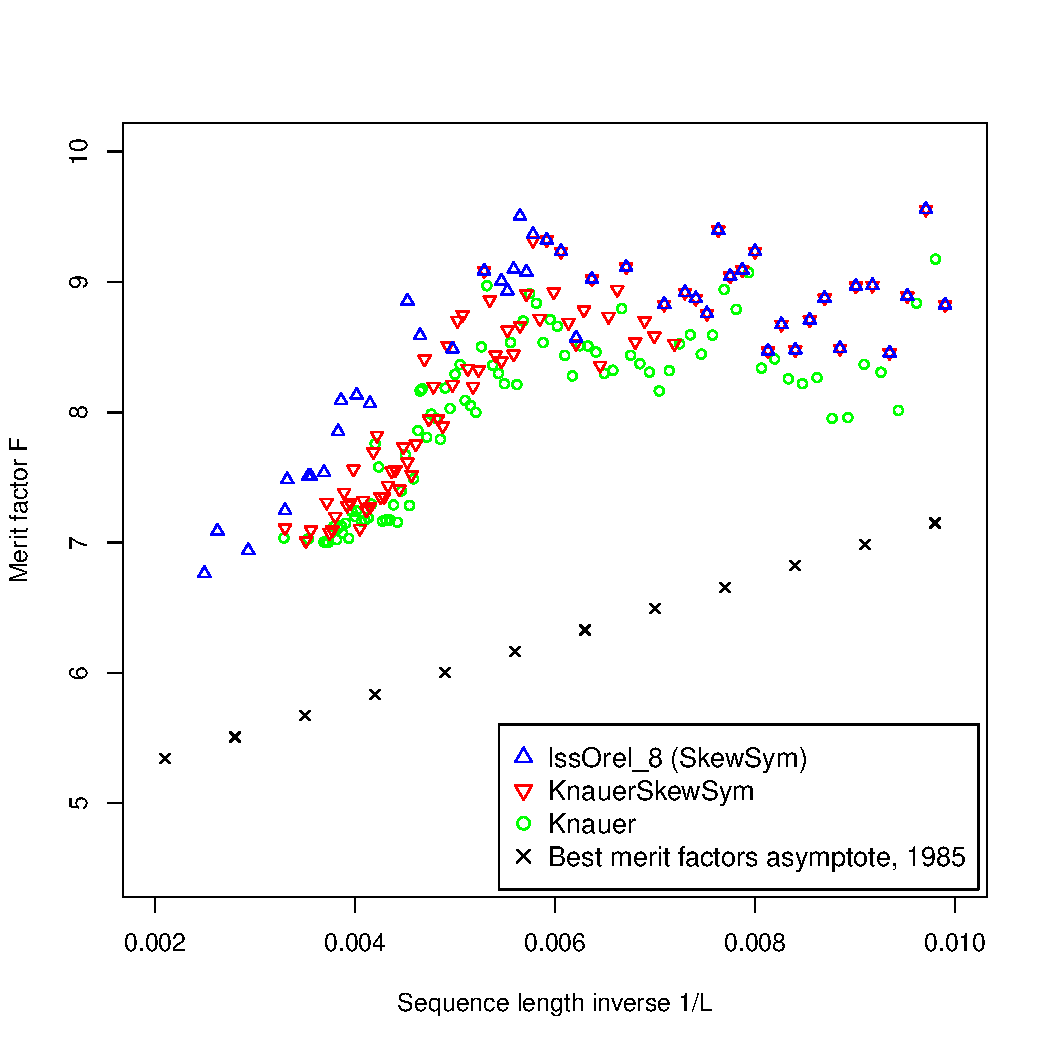
\includegraphics[width=0.99\textwidth]{fg-R-labs-wide-4-figures-c}
\vspace*{-5ex}% removes white space for the next row of figures
\end{minipage}
~%
\begin{minipage}{0.49\textwidth}
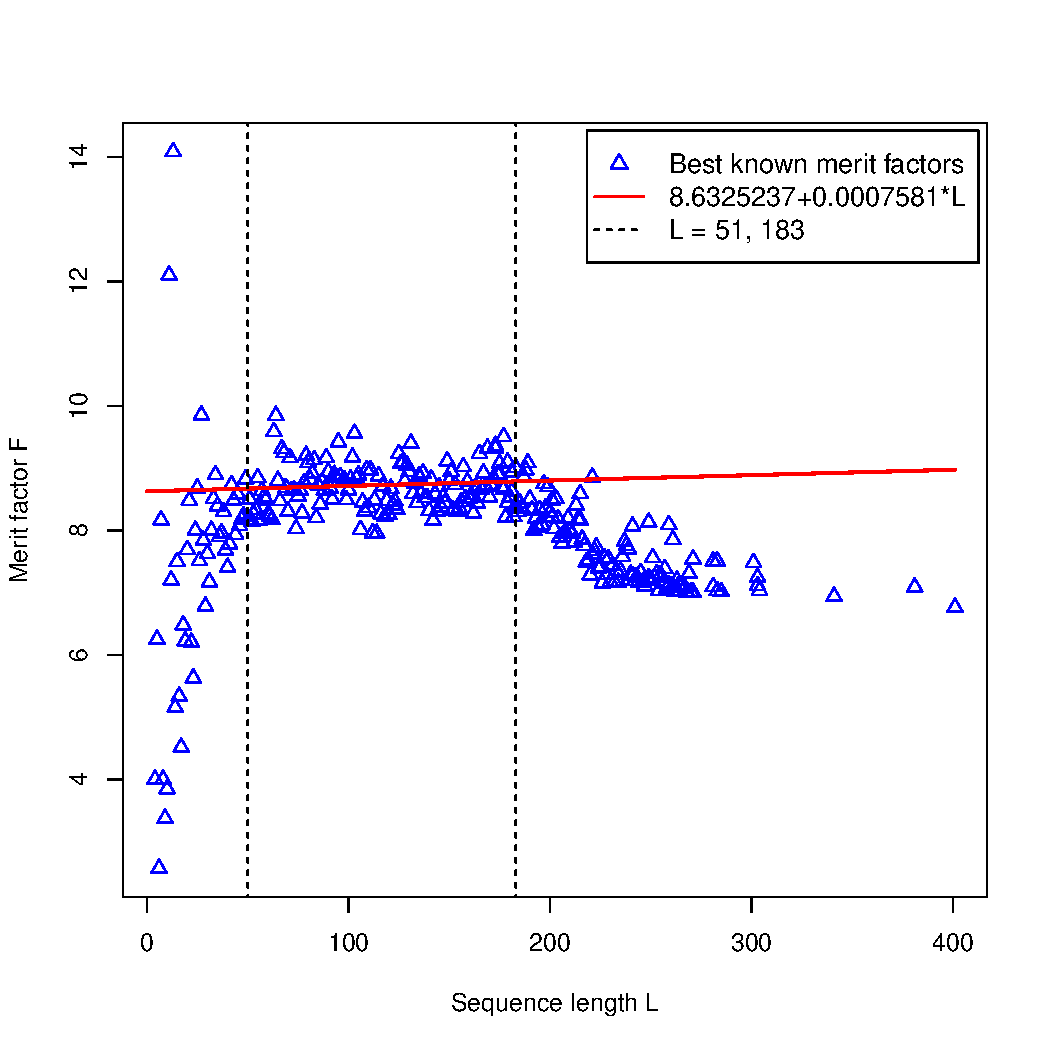
\includegraphics[width=0.99\textwidth]{fg-R-labs-wide-4-figures-d}
%\vspace*{-1ex}
\end{minipage}
%
\begin{minipage}{0.49\textwidth}
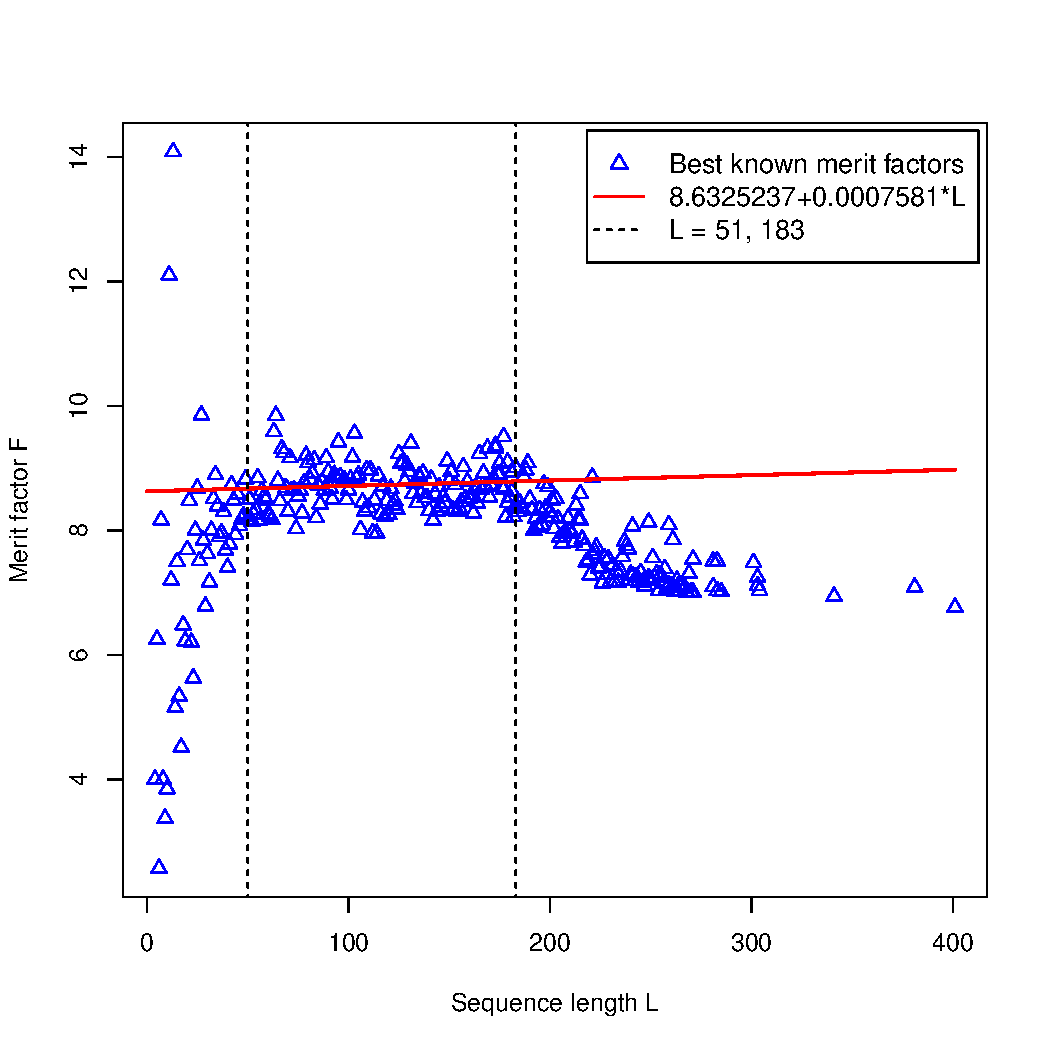
\includegraphics[width=0.99\textwidth]{fg-R-labs-wide-4-figures-d}
%\vspace*{-1ex}
\end{minipage}
%
\caption[From the file fg-R-labs-wide-6-figures.tex]
{From the file fg-R-labs-wide-6-figures.tex {\em borrowed from} {\tt Lib-OPUS2-labs-2015-arxiv-Boskovic}. 
}
\label{fg-R-labs-wide-6-figures}
\end{figure*}




\newthought{The file}  {\tt fg-R-labs-wide-6-figures.tex}  
renders Figure~\ref{fg-R-labs-wide-6-figures}.
\lipsum[1]
\clearpage

\begin{figure}[t!]
% http://en.wikibooks.org/wiki/LaTeX/Floats,_Figures_and_Captions
% http://tex.stackexchange.com/questions/119984/subfigures-side-by-side-with-captions
%\usepackage{caption}     %% loads OK, but not needed neither subfigure nor subcaption
                          %% work under Tufte-book template
%\usepackage{subfigure}   %% This package loads without errors, however 
                          %% \begin{subfigure}[t]{0.49\textwidth} DOES NOT WORK!
%\usepackage{subcaption}  %% ! Package caption Error: The `subcaption' package does not work 
                          %%   correctly in compatibility mode.
\centering
\vspace*{-5ex}% removes white space at the top

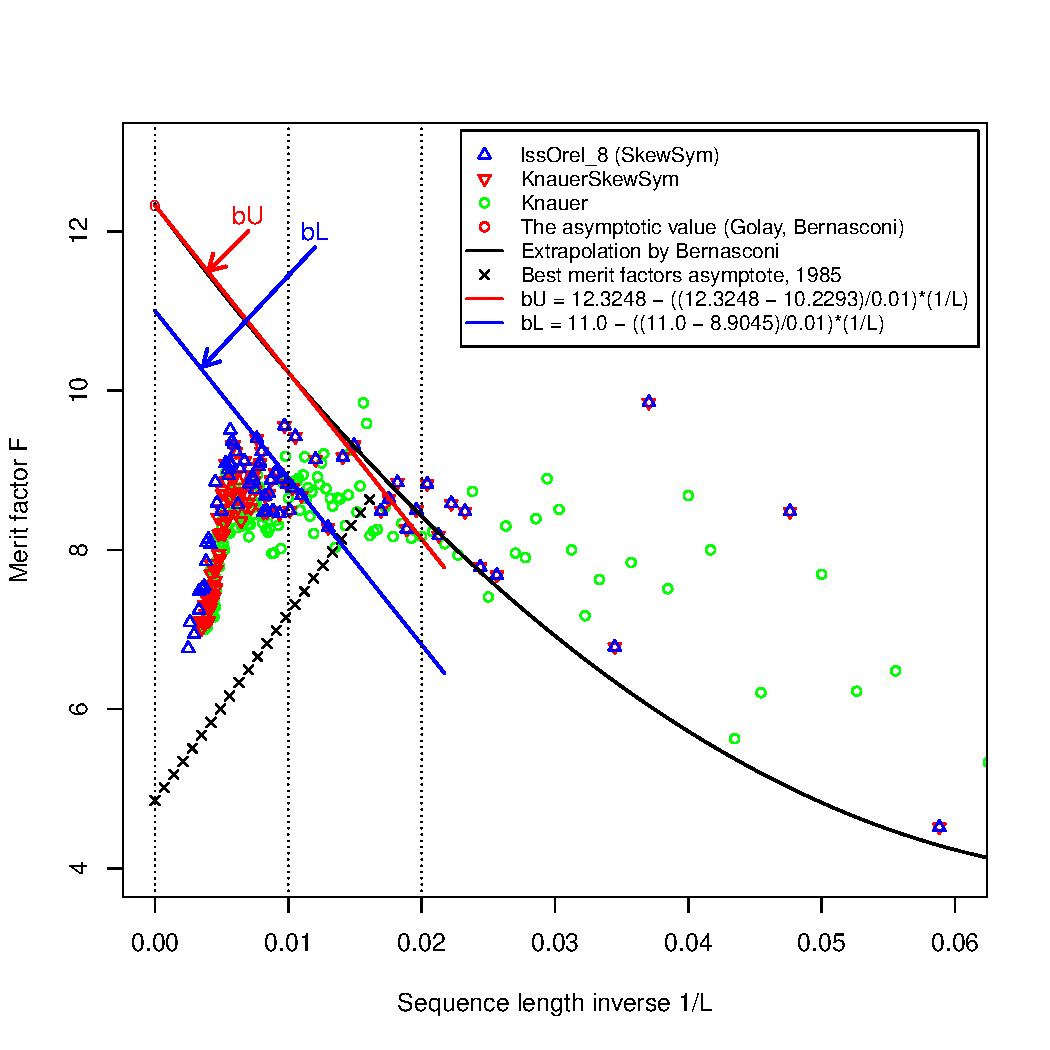
\includegraphics[width=0.79\textwidth]{fg-R-labs-wide-4-figures-b}
\vspace*{-5ex}% removes white space for the next figure 
\\
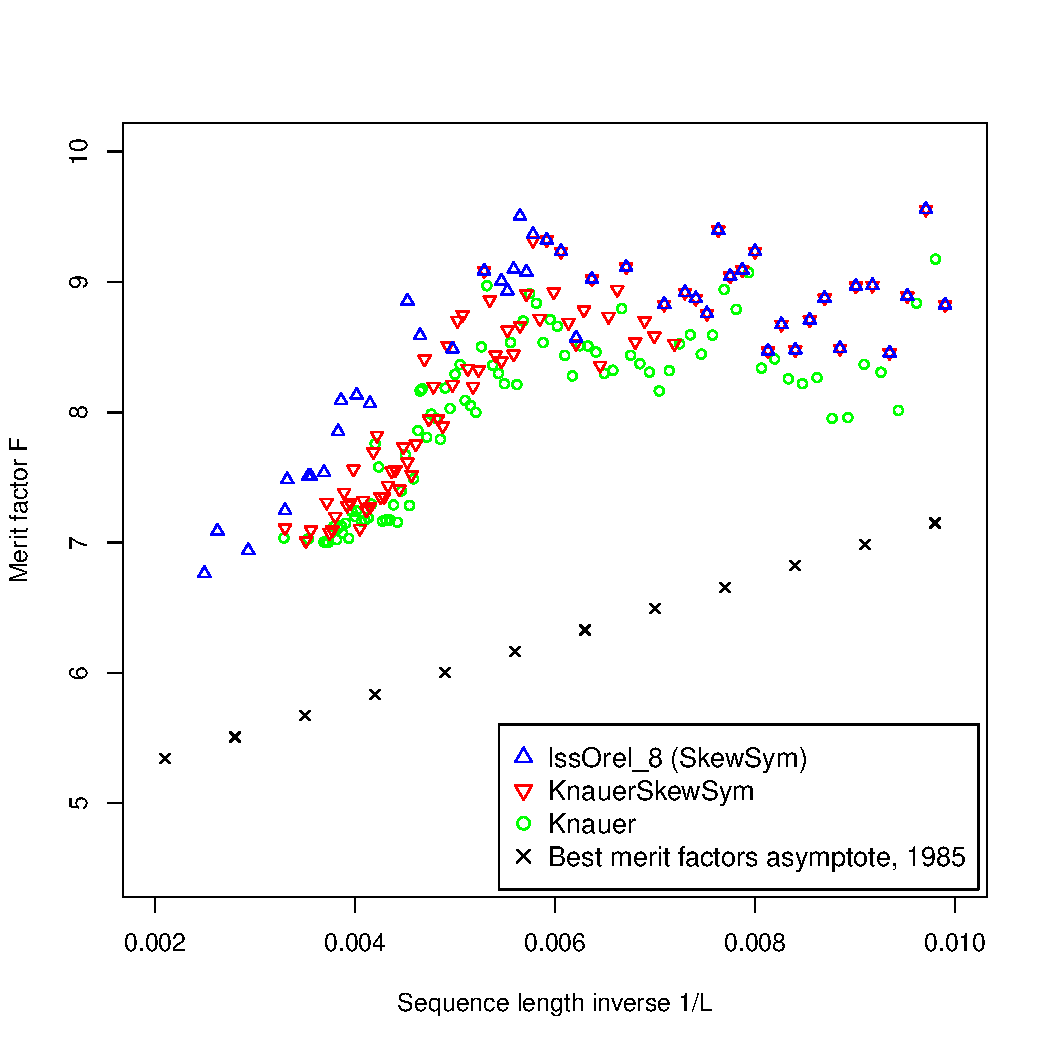
\includegraphics[width=0.79\textwidth]{fg-R-labs-wide-4-figures-c}
\vspace*{-5ex}% removes white space for the next figure 
\\
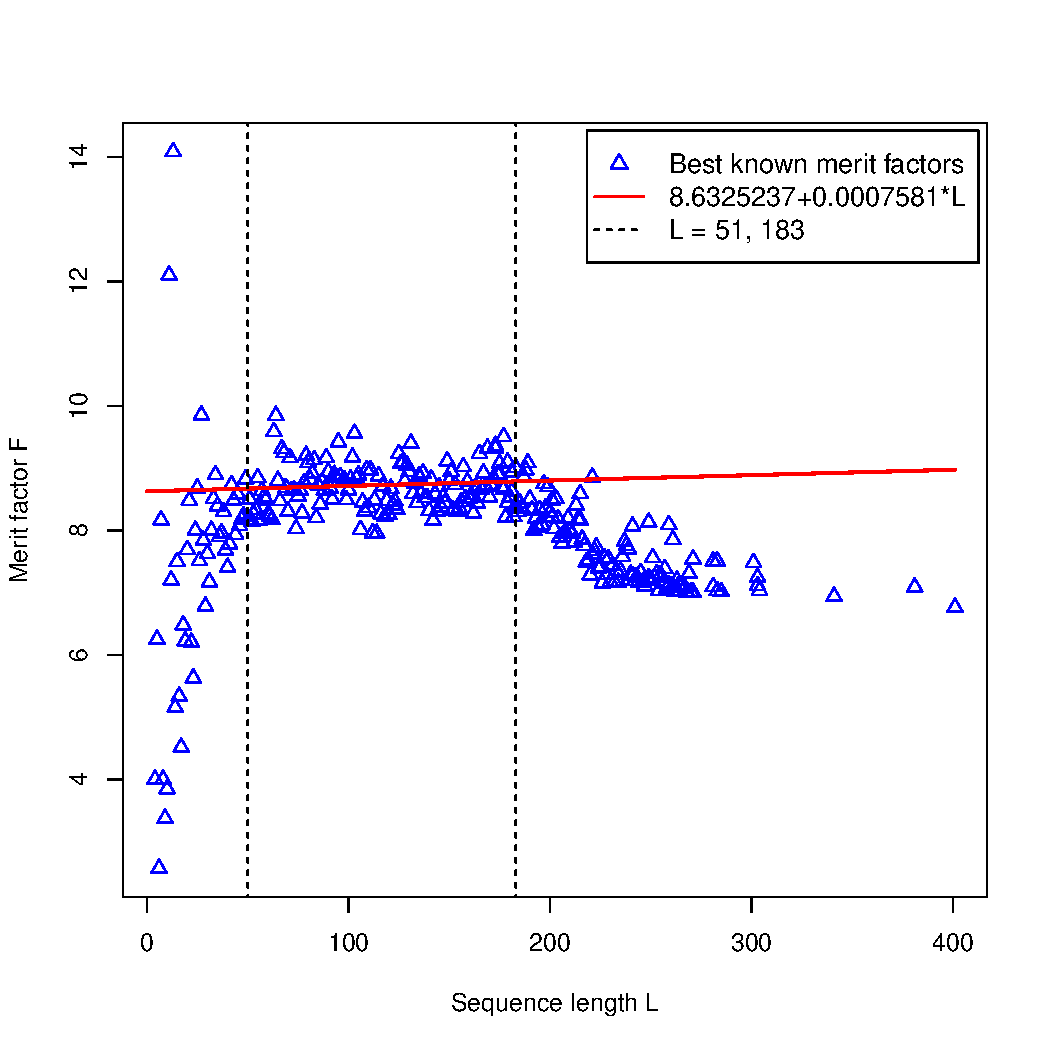
\includegraphics[width=0.79\textwidth]{fg-R-labs-wide-4-figures-d}
\vspace*{-5ex}% removes white space for the next figure 
%
\caption[From the file fg-R-labs-normal-3-figures.tex]
{From the file fg-R-labs-normal-3-figures.tex {\em borrowed from} {\tt Lib-OPUS2-labs-2015-arxiv-Boskovic}.
{\bf NOTE: both `verb' and `cite' commands seem disabled under `figure environment'!}
Also, 3 vertical plots in portrait from R create more white space than the 4 plots 
from R in wide format, see Figure~\ref{fg-R-labs-wide-4-figures}.
Then,
(a) 
it may not be possible to create (a) in this file with \LaTeX ... may need to create it in R;
%
(b)
it may not be possible to create (b) in this file with \LaTeX ... may need to create it in R;
%
(c)
it may not be possible to create (c) in this file with \LaTeX ... may need to create it in R.
}
\label{fg-R-labs-normal-3-figures}
\end{figure}



\newthought{The file}  {\tt fg-R-labs-normal-3-figures.tex}  
renders Figure~\ref{fg-R-labs-normal-3-figures}.
{\bf NOTE AGAIN: both `verb' and `cite' commands seem disabled under `figure environment'!}
\lipsum[2]

\begin{figure}[t!]
% http://en.wikibooks.org/wiki/LaTeX/Floats,_Figures_and_Captions
% http://tex.stackexchange.com/questions/119984/subfigures-side-by-side-with-captions
%\usepackage{caption}     %% loads OK, but not needed neither subfigure nor subcaption
                          %% work under Tufte-book template
%\usepackage{subfigure}   %% This package loads without errors, however 
                          %% \begin{subfigure}[t]{0.49\textwidth} DOES NOT WORK!
%\usepackage{subcaption}  %% ! Package caption Error: The `subcaption' package does not work 
                          %%   correctly in compatibility mode.
\centering
\vspace*{-0ex}% removes white space at the top

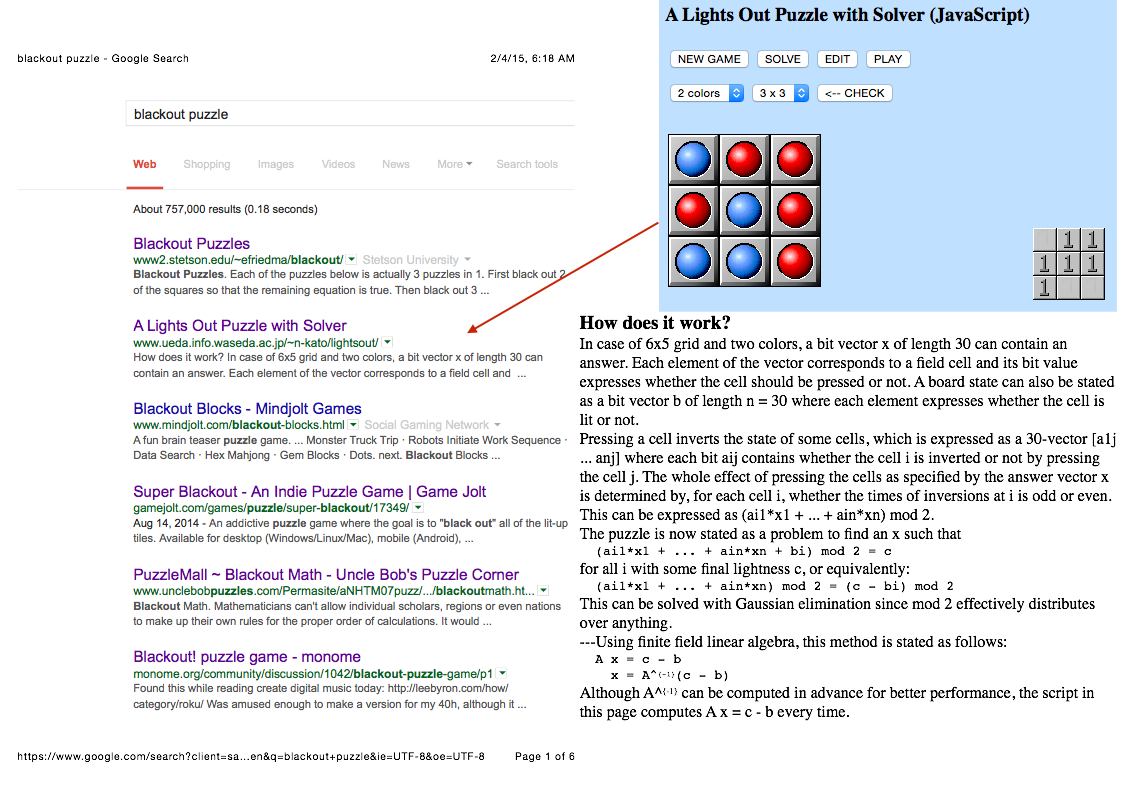
\includegraphics[width=0.99\textwidth]{fg-key-blackp-descr-a}
\vspace*{1ex}% removes white space for the next figure 
\\
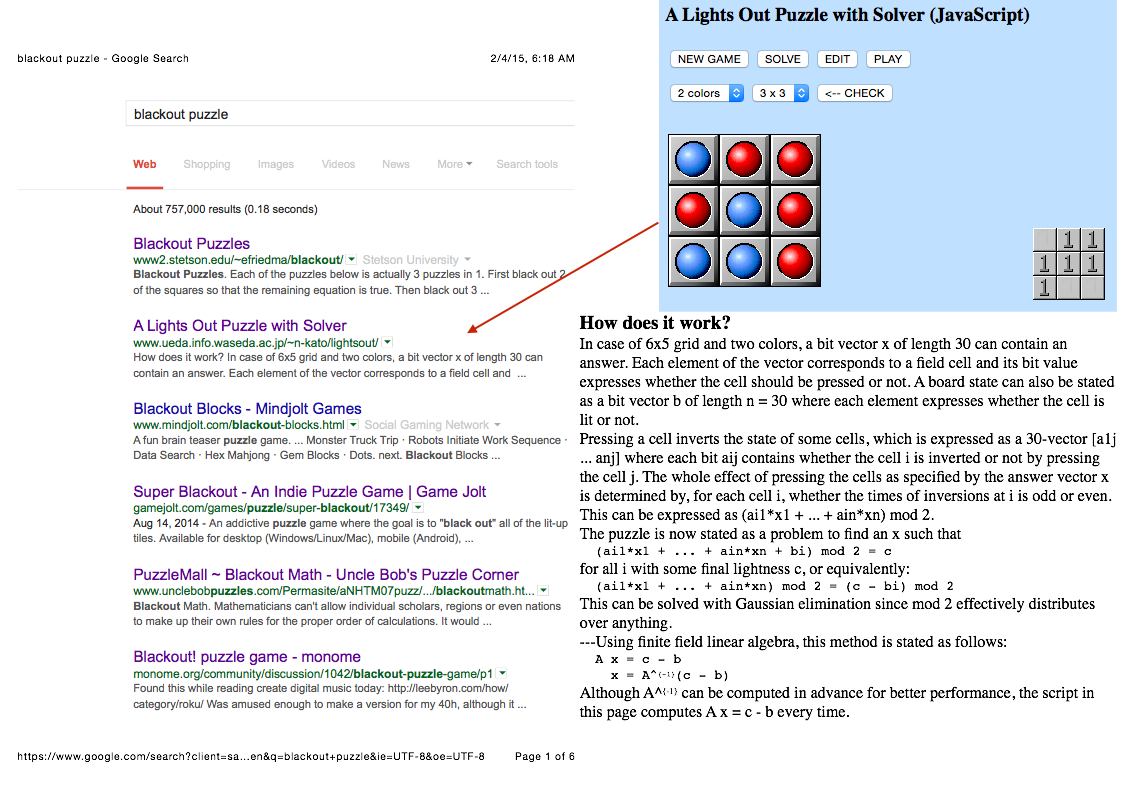
\includegraphics[width=0.99\textwidth]{fg-key-blackp-descr-a}
\vspace*{1ex}% removes white space for the next figure 
\\
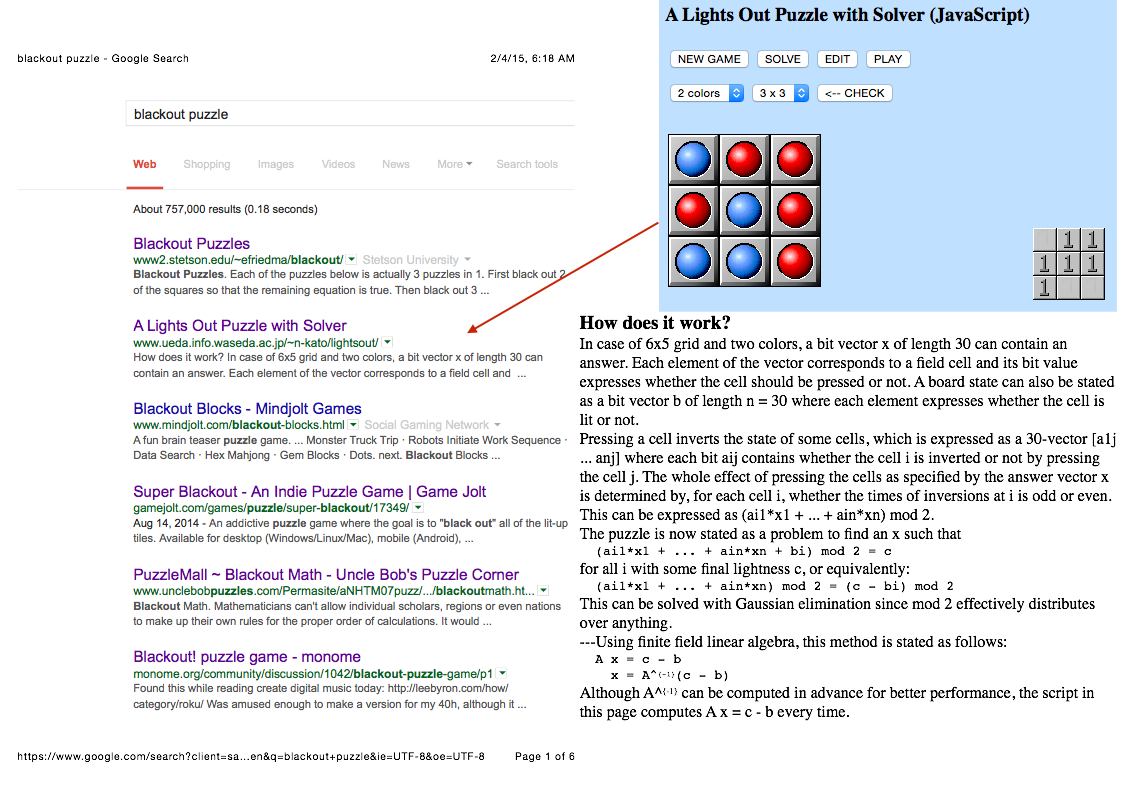
\includegraphics[width=0.99\textwidth]{fg-key-blackp-descr-a}
\vspace*{1ex}% removes white space for the next figure 
%
% https://github.com/fbrglez/gitPublic/tree/master/xProj499-Sp15
\caption[From the file fg-key-blackp-normal-3-figures.tex]
{From the file fg-key-blackp-portrait-3-figures.tex {\em borrowed from} {\tt Lib-OPUS2-ebook-CSC499-Sp15-2015-Brglez}.
{\bf NOTE: both `verb' and `cite' commands seem disabled under `figure environment'!}
Also, the portrait of 3 plots from Keynote are larger than the 3 plots from R in portrait format,
see Figure~\ref{fg-R-labs-portrait-3-figures}.
Then,
(a) 
it may not be possible to create (a) in this file with \LaTeX ... may need to create it in Keynote;
%
(b)
it may not be possible to create (b) in this file with \LaTeX ... may need to create it in Keynote;
%
(c)
it may not be possible to create (c) in this file with \LaTeX ... may need to create it in Keynote.
}
\label{fg-key-blackp-normal-3-figures}
\end{figure}



\newthought{The file}
fg-key-blackp-normal-3-figures, first used 
in\cite[27ex]{Lib-OPUS2-ebook-CSC499-Sp15-2015-Brglez},
renders Figure~\ref{fg-key-blackp-normal-3-figures}.
\lipsum[3]

\begin{figure}[h!]

\centering
\vspace*{-0ex}% removes white space at the top
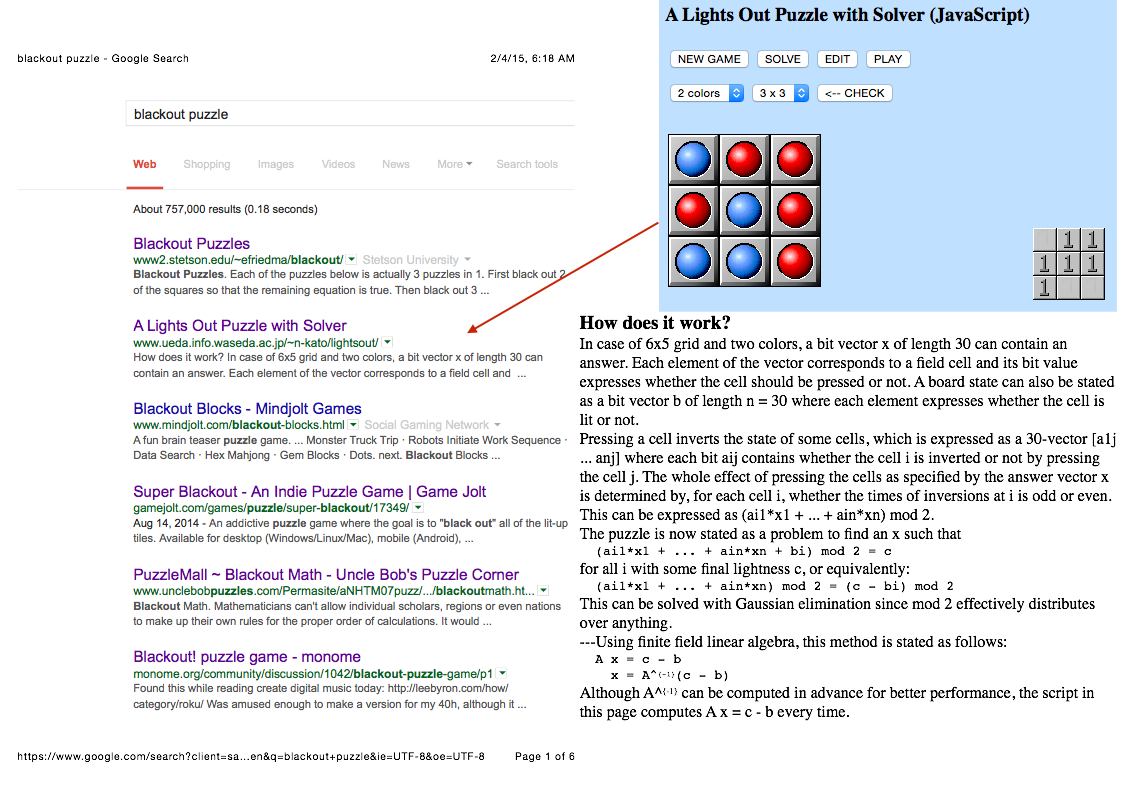
\includegraphics[width=0.85\textwidth]{fg-key-blackp-descr-a}

\caption[From the file fg-key-blackp-normal-1-figures.tex]
{From the file fg-key-blackp-normal-2-figures.tex {\em borrowed from} {\tt Lib-OPUS2-ebook-CSC499-Sp15-2015-Brglez}.
{\bf NOTE: both `verb' and `cite' commands seem disabled under `figure environment'!}
}
\label{fg-key-blackp-normal-1-figure}
\end{figure}



\begin{figure}[h!]

\centering
\vspace*{-0ex}% removes white space at the top
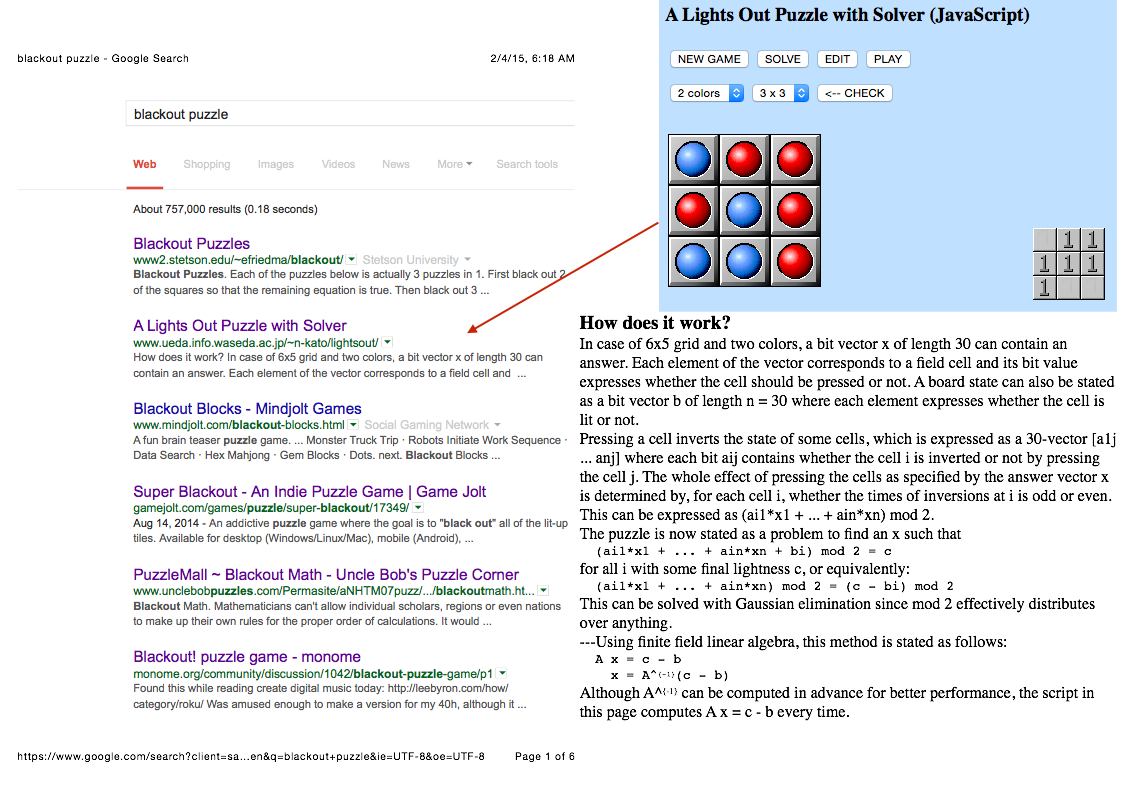
\includegraphics[width=0.85\textwidth]{fg-key-blackp-descr-a}

\caption[From the file fg-key-blackp-normal-1-figures.tex]
{From the file fg-key-blackp-normal-2-figures.tex {\em borrowed from} {\tt Lib-OPUS2-ebook-CSC499-Sp15-2015-Brglez}.
{\bf NOTE: both `verb' and `cite' commands seem disabled under `figure environment'!}
}
\label{fg-key-blackp-normal-1-figure}
\end{figure}



\begin{figure}[h!]

\centering
\vspace*{-0ex}% removes white space at the top
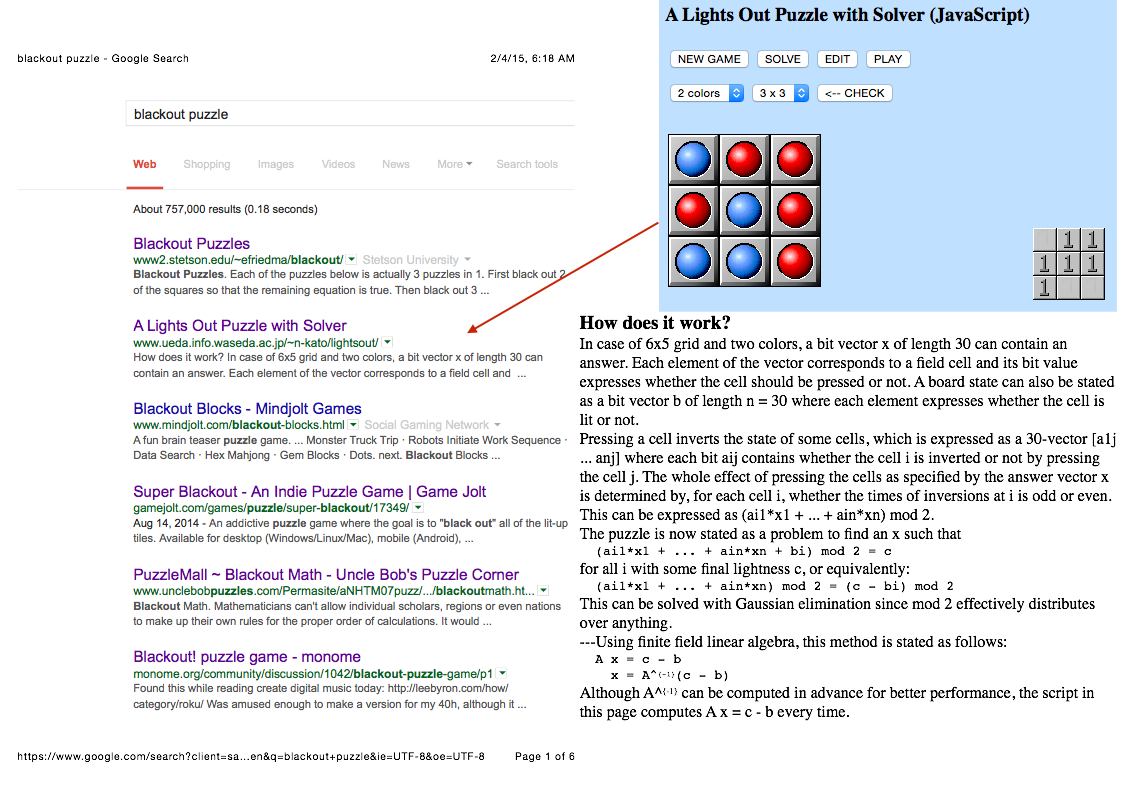
\includegraphics[width=0.85\textwidth]{fg-key-blackp-descr-a}

\caption[From the file fg-key-blackp-normal-1-figures.tex]
{From the file fg-key-blackp-normal-2-figures.tex {\em borrowed from} {\tt Lib-OPUS2-ebook-CSC499-Sp15-2015-Brglez}.
{\bf NOTE: both `verb' and `cite' commands seem disabled under `figure environment'!}
}
\label{fg-key-blackp-normal-1-figure}
\end{figure}




\newthought{The file}
fg-key-blackp-normal-1-figure.tex  
renders Figure~\ref{fg-key-blackp-normal-1-figure}.
\lipsum[4]
\lipsum[4]


\clearpage
\newthought{The file}
fg-key-blackp-wide-1-figure.tex, 
renders Figure~\ref{fg-key-blackp-wide-1-figure}.

\begin{figure*}[t!]

\centering
\vspace*{-0ex}% removes white space at the top
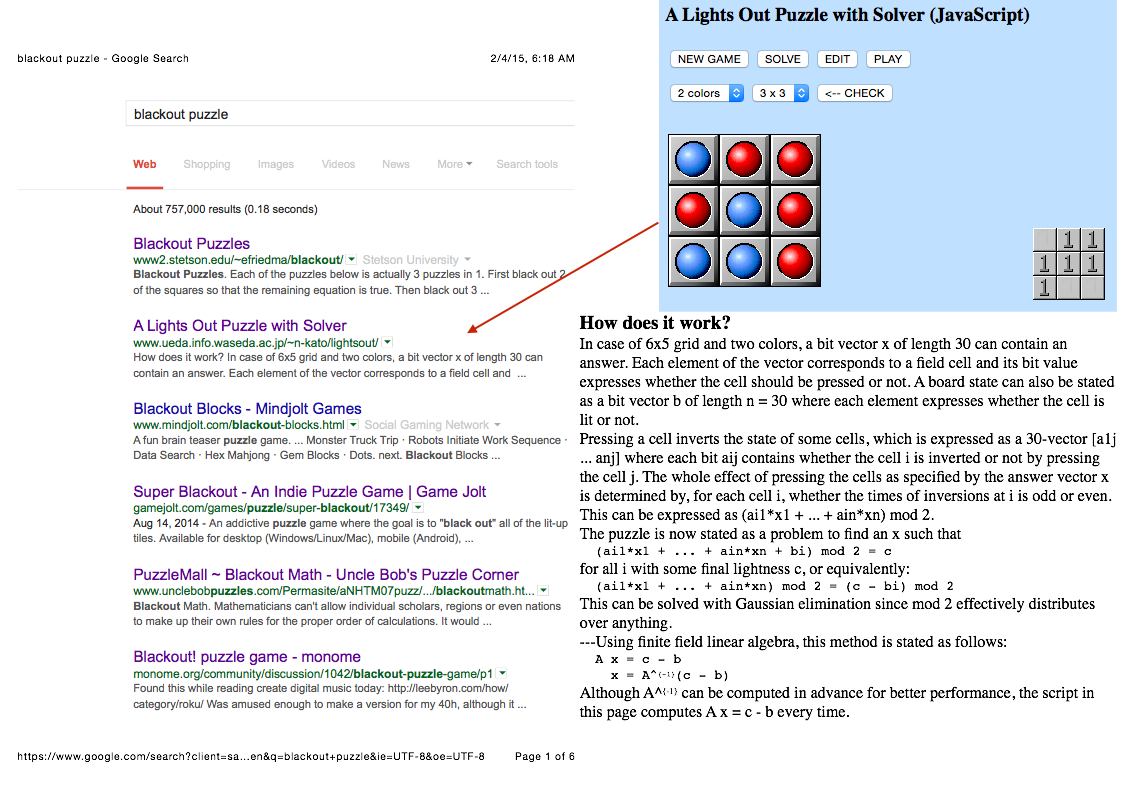
\includegraphics{fg-key-blackp-descr-a}

\caption[From the file fg-key-blackp-wide-1-figures.tex]
{From the file fg-key-blackp-wide-1-figures.tex {\em borrowed from} {\tt Lib-OPUS2-ebook-CSC499-Sp15-2015-Brglez}.
}
\label{fg-key-blackp-wide-1-figure}
\end{figure*}




\lipsum[4]
\begin{figure*}[t!]

\centering
\vspace*{-0ex}% removes white space at the top
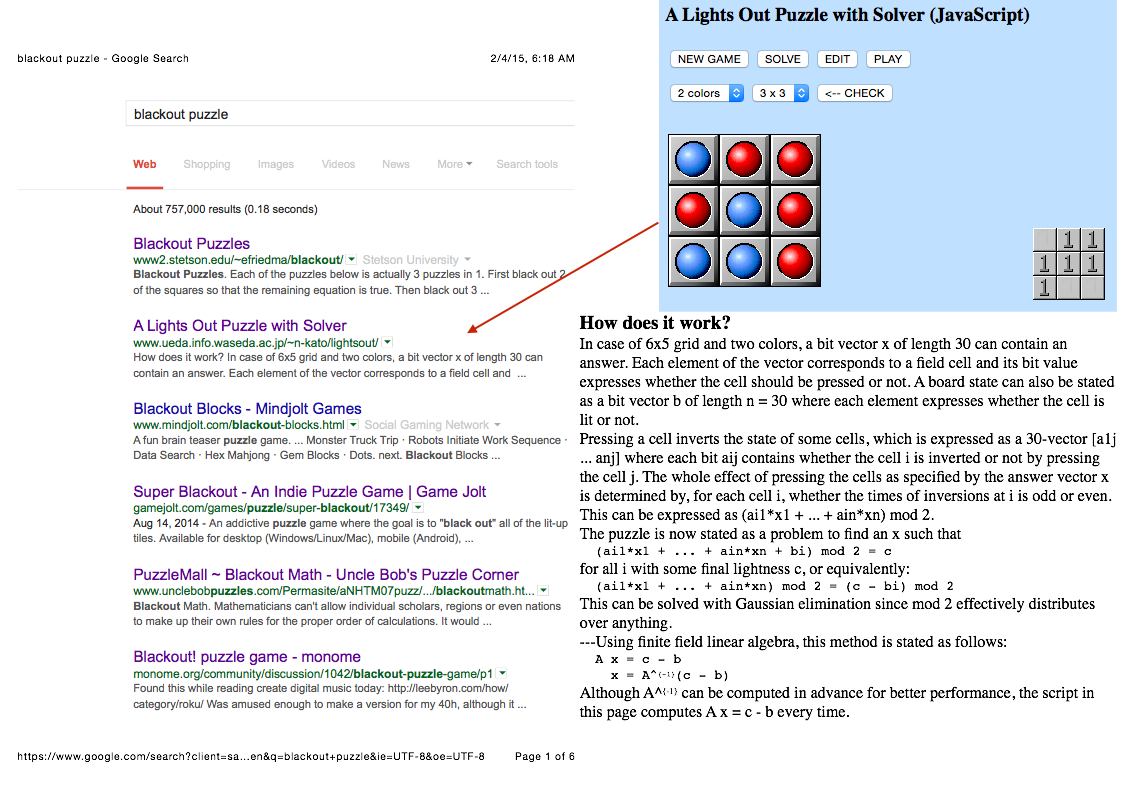
\includegraphics[width=0.90\textwidth]{fg-key-blackp-descr-a}
\\[3ex]
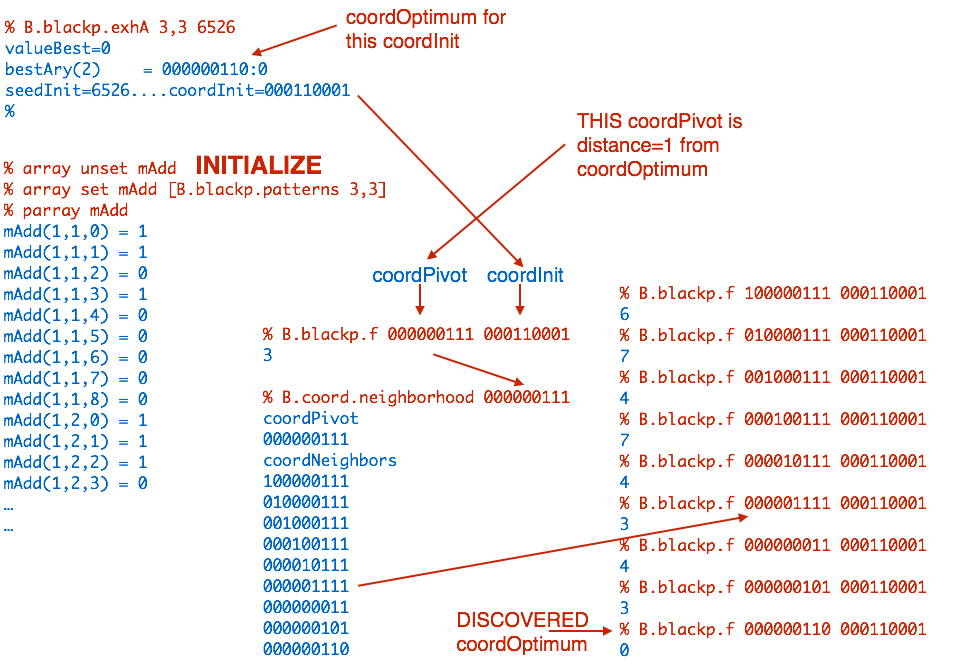
\includegraphics[width=0.90\textwidth]{fg-key-blackp-neighbors}

\caption[From the file fg-key-blackp-wide-2-figures.tex]
{From the file fg-key-blackp-wide-2-figures.tex {\em borrowed from} {\tt Lib-OPUS2-ebook-CSC499-Sp15-2015-Brglez}.
}
\label{fg-key-blackp-wide-2-figures}
\end{figure*}



\newthought{The file}
fg-key-blackp-wide-2-figures.tex  
renders Figure~\ref{fg-key-blackp-wide-2-figures}.
The file
fg-key-blackp-wide-2-figures.tex  
renders Figure~\ref{fg-key-blackp-wide-2-figures}.
The file
fg-key-blackp-wide-2-figures.tex  
renders Figure~\ref{fg-key-blackp-wide-2-figures}.
The file
fg-key-blackp-wide-2-figures.tex  
renders Figure~\ref{fg-key-blackp-wide-2-figures}.
The file
fg-key-blackp-wide-2-figures.tex  
renders Figure~\ref{fg-key-blackp-wide-2-figures}.
The file
fg-key-blackp-wide-2-figures.tex  
renders Figure~\ref{fg-key-blackp-wide-2-figures}.
The file
fg-key-blackp-wide-2-figures.tex  
renders Figure~\ref{fg-key-blackp-wide-2-figures}.

\clearpage
\begin{figure*}[t!]

\centering
\vspace*{-5ex}% removes white space at the top

\begin{minipage}{0.49\textwidth}
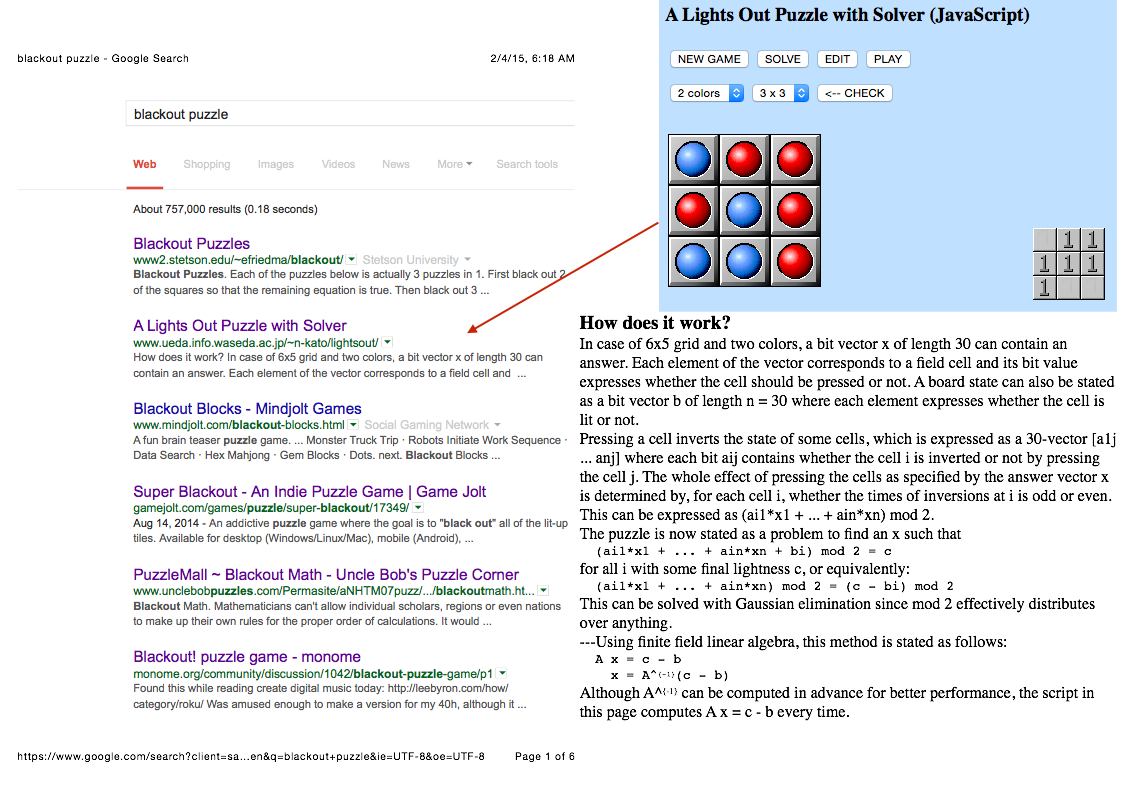
\includegraphics[width=0.95\textwidth]{fg-key-blackp-descr-a}
\vspace*{+2ex}% removes white space for the next row of figures
\end{minipage}
\begin{minipage}{0.49\textwidth}
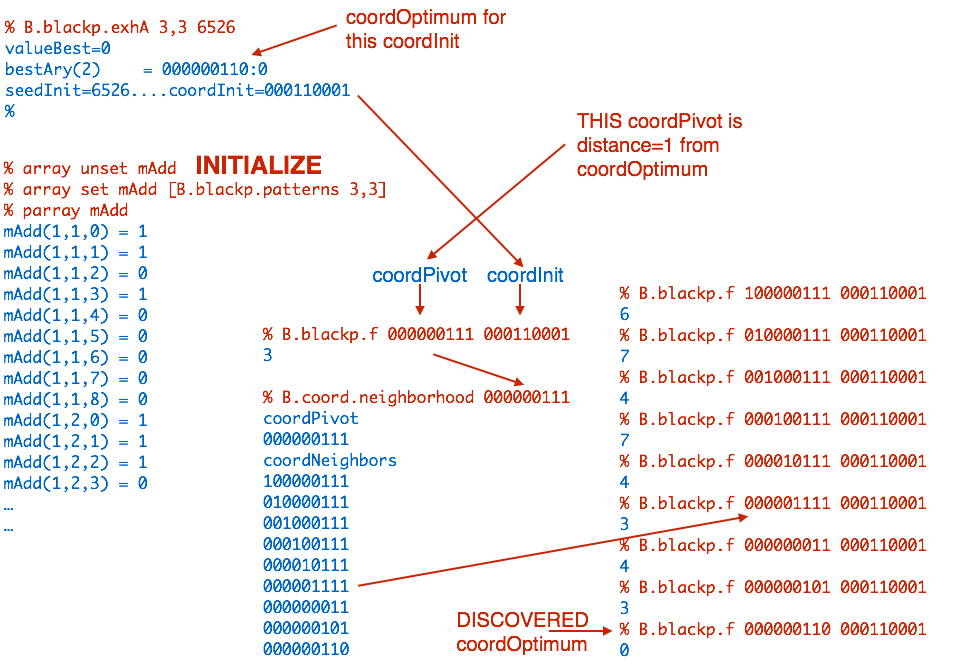
\includegraphics[width=0.95\textwidth]{fg-key-blackp-neighbors}
\vspace*{+2ex}% removes white space for the next row of figures
\end{minipage}
~%
\begin{minipage}{0.49\textwidth}
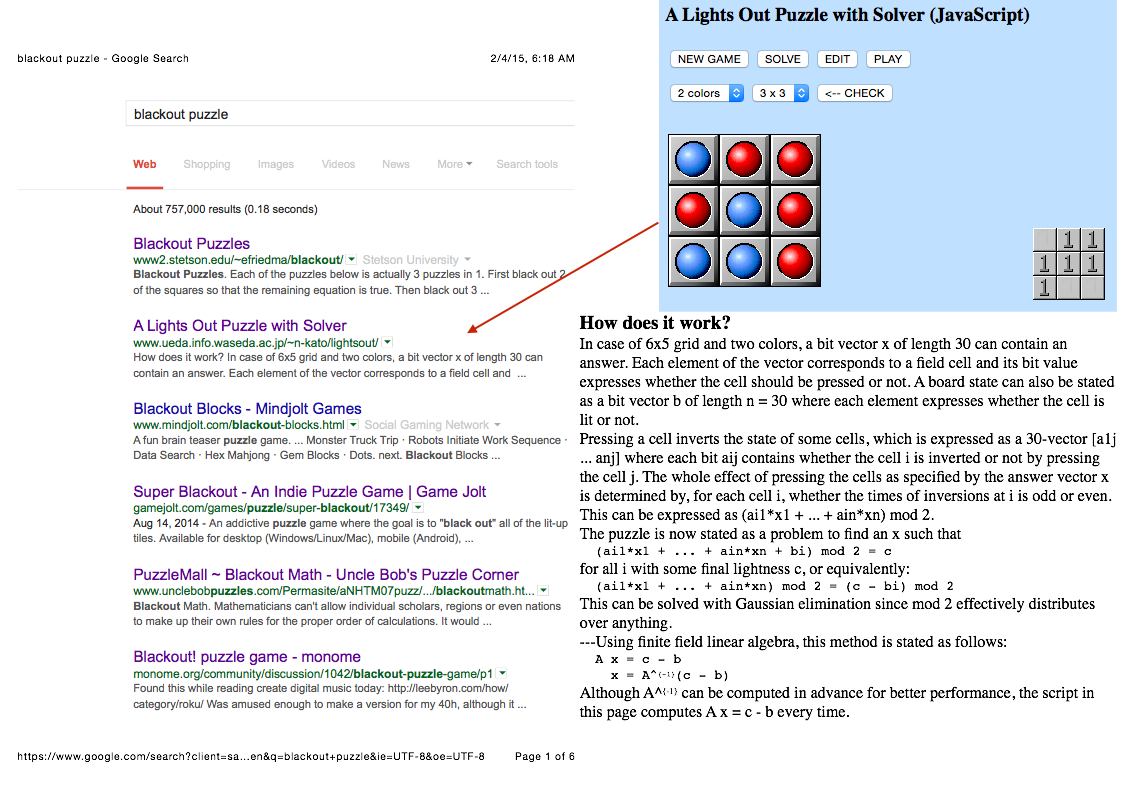
\includegraphics[width=0.95\textwidth]{fg-key-blackp-descr-a}
%\vspace*{+1ex}
\end{minipage}
%
\begin{minipage}{0.49\textwidth}
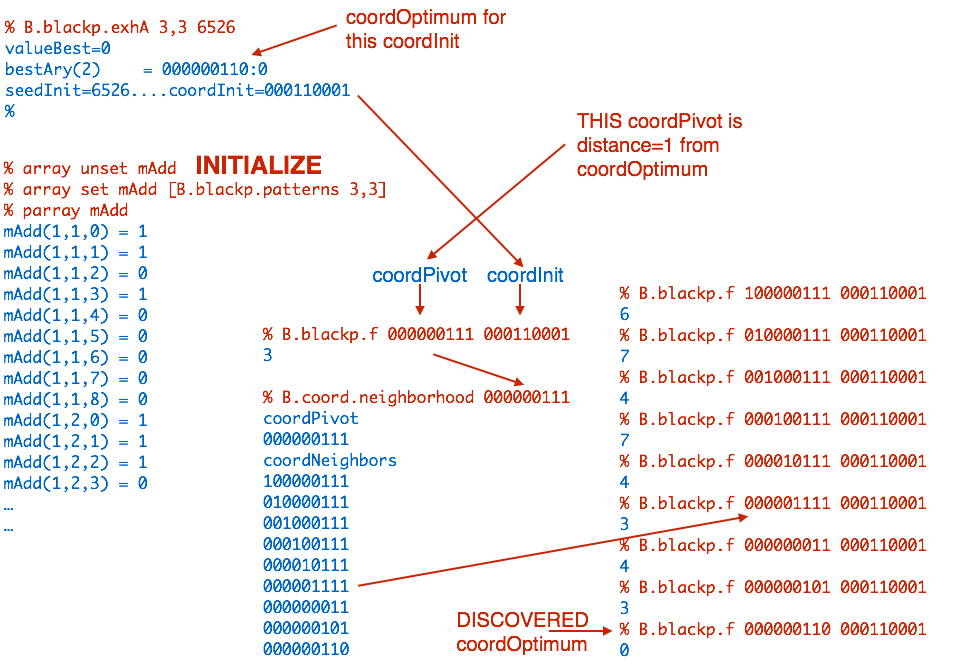
\includegraphics[width=0.95\textwidth]{fg-key-blackp-neighbors}
%\vspace*{-1ex}
\end{minipage}

\caption[From the file fg-key-blackp-wide-4-figures.tex][4ex]
{From the file fg-key-blackp-wide-4-figures.tex {\em borrowed from} {\tt Lib-OPUS2-ebook-CSC499-Sp15-2015-Brglez}.
}
\label{fg-key-blackp-wide-4-figures}
\end{figure*}


\newthought{The file }
fg-key-blackp-wide-4-figures.tex, 
renders Figure~\ref{fg-key-blackp-wide-4-figures}.
\lipsum[4]
\lipsum[4]


\chapter{About Tables}
\label{chap-Tables}
\newthought{Tables in this chapter} are divided into two sections: 
(1) tables from Tufte,
(2) tables from other sources.

\newthought{For details} about how various text items are being represented,
see Chapter~\ref{chap-About}.

%\chapter{About Tables}
%\label{chap-Tables}
%\newthought{Tables in this chapter} are divided into two sections: 
%(1) tables from Tufte,
%(2) tables from other sources.
%
\section{Tables from Tufte}
\label{chap-Tables-Tufte}

\newthought{About the tables}  from Tufte:
\lipsum[4]
\begin{itemize}
\item
a normal-width table, {\tt tb-tufte-normal-headings}, Table~\ref{tb-tufte-normal-headings}, 
\item
a normal-width table, {\tt tb-tufte-normal-fontSizes}, Table~\ref{tb-tufte-normal-fontSizes},
\item
a normal-width table, {\tt tb-tufte-normal-environmentStyles}, Table~\ref{tb-tufte-normal-environmentStyles},  
\item
a normal-width table, {\tt tb-tufte-normal-environmentStyles}, Table~\ref{tb-tufte-normal-margins}, and
\item
a wide table, {\tt tb-tufte-wide-extraColumn}, Table~\ref{tb-tufte-wide-extraColumn}.
\end{itemize}
%\lipsum[4]
\begin{table}[h]
  \begin{center}
    \footnotesize%
    \begin{tabular}{lcr}
      \toprule
      Heading & Style & Size \\
      \midrule
      Part & roman & \measure{24}{36}{40} \\
      Chapter & italic & \measure{20}{30}{40} \\
      Section & italic & \measure{12}{16}{26} \\
      Subsection & italic & \measure{11}{15}{26} \\
      Paragraph & italic & 10/14 \\
      \bottomrule
    \end{tabular}
  \end{center}
  \caption[From the file tb-tufte-normal-headings.tex][0ex]
  {Heading styles used in \BE.}
  \label{tb-tufte-normal-headings}
\end{table}

\begin{table}[h]\index{typefaces!sizes}
  \footnotesize%
  \begin{center}
    \begin{tabular}{lccl}
      \toprule
      \LaTeX{} size & Font size & Leading & Used for \\
      \midrule
      \verb+\tiny+         &  5 &  6 & sidenote numbers \\
      \verb+\scriptsize+   &  7 &  8 & \na \\
      \verb+\footnotesize+ &  8 & 10 & sidenotes, captions \\
      \verb+\small+        &  9 & 12 & quote, quotation, and verse environments \\
      \verb+\normalsize+   & 10 & 14 & body text \\
      \verb+\large+        & 11 & 15 & \textsc{b}-heads \\
      \verb+\Large+        & 12 & 16 & \textsc{a}-heads, \textsc{toc} entries, author, date \\
      \verb+\LARGE+        & 14 & 18 & handout title \\
      \verb+\huge+         & 20 & 30 & chapter heads \\
      \verb+\Huge+         & 24 & 36 & part titles \\
      \bottomrule
    \end{tabular}
  \end{center}
  \caption[From the file tb-tufte-normal-fontSizes][0ex]
  {A list of \LaTeX{} font sizes as defined by the \TL document classes.}
  \label{tb-tufte-normal-fontSizes}
\end{table}

\begin{table}[h]
  \begin{center}
    \footnotesize%
    \begin{tabular}{lcl}
      \toprule
      Environment & Font size & Notes \\
      \midrule
      Body text & \measure{10}{14}{26} & \\
      Block quote & \measure{9}{12}{24} & Block indent (left and right) by \unit[1]{pc} \\
      Sidenotes & \measure{8}{10}{12} & Sidenote number is set inline, followed by word space \\
      Captions & \measure{8}{10}{12} &  \\
      \bottomrule
    \end{tabular}
  \end{center}
  \caption[From the file tb-tufte-normal-environmentStyles.tex][0ex]
  {Environment styles used in \BE.}
  \label{tb-tufte-normal-environmentStyles}
\end{table}

\begin{table}[h]
  \centering
  \fontfamily{ppl}\selectfont
  \begin{tabular}{ll}
    \toprule
    Margin & Length \\
    \midrule
    Paper width & \unit[8\nicefrac{1}{2}]{inches} \\
    Paper height & \unit[11]{inches} \\
    Textblock width & \unit[6\nicefrac{1}{2}]{inches} \\
    Textblock/sidenote gutter & \unit[\nicefrac{3}{8}]{inches} \\
    Sidenote width & \unit[2]{inches} \\
    \bottomrule
  \end{tabular}
  \caption[From the file tb-tufte-normal-margins.tex][0ex]
  {Here are the dimensions of the various margins used in the Tufte-handout class.}
  \label{tb-tufte-normal-margins}
  %\zsavepos{pos:normaltab}
\end{table}

\begin{table*}[h]
  \begin{center}
    \footnotesize%
    \begin{tabular}{lclr}
      \toprule
      Environment & Font size & Notes & Extra column\\
      \midrule
      Body text   & \measure{10}{14}{26} &                                                       & Whatever we need etc, etc, etc, etc, etc ...\\
      Block quote & \measure{9}{12}{24}  & Block indent (left and right) by \unit[1]{pc}         & \\
      Sidenotes   & \measure{8}{10}{12}  & Sidenote number is set inline, followed by word space & \\
      Captions   & \measure{8}{10}{12}   &                                                       &  Another item here ...   \\
      \bottomrule
    \end{tabular}
  \end{center}
  \caption[From the file tb-tufte-wide-extraColumn.tex][3ex]
  {Environment styles modifications used in \BE ....}
  \label{tb-tufte-wide-extraColumn}
\end{table*}

%\chapter{About Tables}
%\label{chap-Tables}
%\newthought{Tables in this chapter} are divided into two sections: 
%(1) tables from Tufte,
%(2) tables from other sources.
%

\clearpage
\section{Tables from Other Sources}
\label{chap-Tables-Other}

\newthought{About the tables}  from other sources:
\lipsum[4]
\begin{itemize}
\item
a wide table, {\tt tb-tufte-wide-extraColumn}, Table~\ref{tb-tufte-wide-extraColumn}
from\cite[2ex]{Lib-OPUS2-ebook-xBed-2015-Brglez,Lib-OPUS2-labs-2015-arxiv-Boskovic}, and
\item
a sideways table, {\tt tb-cover-sideways-results}, Table~\ref{tb-cover-sideways-results}.\\{\bf NOTE: to get the table number printed here, we had to move
the label AFTER the caption!!!}.
\end{itemize}
\lipsum[4]

\begin{table*}[t]\index{xBed!notation}
\footnotesize%
\caption[From the file tb-labs-wide-notation-summary.tex][3ex]
{Summary of notation: symbols, names, and descriptions.}
\label{tb-labs-wide-notation-summary}
\centering
\begin{tabular}[]{c c}
\begin{tabular}[t]{l l l}  
\centering
\bf{symbol}  & \bf{short name} & \bf{brief description} \\ \hline\\[-1.25ex]
$L$ & coordDim & instance size \\[1.25ex]
%$\lambda$ & laevusNumber & coord. prefix size \\[0.95ex]
$L'$ & coordDim'& instance size under  \\[-0.25ex]
      &          &  skew-symmetry   \\[-0.25ex]
%     &          &  coord. prefix size: \\%[0.95ex]
      &          &  $(L+1)/2 $ \\[1.25ex]
$\sigma_0$ &  seedInit     &  initial seed integer \\[1.05ex]
${\underline \varsigma}_0$ & coordInit & initial coordinate \\[1.05ex]
$\Theta({\underline \varsigma}_0)$ & valueInit & initial value \\[1.05ex]
${\underline \varsigma}_j$ & coordPivot & pivot coordinate\\[1.75ex]
$\Theta({\underline \varsigma}_j)$ & valuePivot & pivot value \\[1.75ex]
${\underline \varsigma}_j^i$ & coordNeighb & pivot neighbor coord. \\[1.75ex] %${\underline \varsigma}_j^i$ \\[1.55ex] 
${\cal N} ({\underline \varsigma}_j)$ & coordNeighbSet & full neighborhood set \\[-0.45ex] %complete \\[-0.95ex] 
                                      &                & of pivot coordinate \\[1.75ex] 
{${\cal N}_{saw} ({\underline \varsigma}_j)$} & {sawNeighbSet} & {SAW neighborhood set} \\[+1.15ex] 
$\omega_c$     & walkSegmCoef &  walk segment coefficient\\[+01.20ex]  
$\omega_{lmt} = \omega_c \times L' $ & walkSegmLmt & walk segm. length limit\\[1.75ex] 
{$Walk_{\omega} ~= $}  & {~~~} & {~~~} \\[0.25ex]
~~=~$\{{\underline \varsigma}_0, \dots , {\underline \varsigma}_\omega\}$ 
& walkList & walk list after $\omega$ steps \\[3.50ex]
%$t$ & runtime & CPU runtime  \\[0.45ex] 
%$t_{lmt}$ & runtimeLmt & solver timeout value\\ 
%$\tau$ & cntProbe & \# of function probes \\% (f. evals) \\  
%$\rho$ & cntRestart & \# of walk restarts  \\[0.45ex] 
\hline
\multicolumn{3}{l}{ }  \\[-1.0ex]
\multicolumn{3}{l}{For \labs\ problems with an odd value of $L$, $L' = (L+1)/2 $}  \\ 
\multicolumn{3}{l}{represents a {\em de facto} instance size under skew-symmetry.}  \\ 
\end{tabular}
&% 
\begin{tabular}[t]{ l l l} 
\centering
\bf{symbol}  & \bf{short name} & \bf{brief description} \\ \hline\\[-1.25ex]
$t$ & runtime & CPU runtime  \\[0.35ex]  
$t_{lmt}$ & runtimeLmt & solver timeout value\\[0.35ex]  
$\tau$ & cntProbe & \# of function probes \\[0.35ex] % (f. evals)   
$\rho$ & cntRestart & \# of walk restarts  \\[0.35ex]  
$ \beta $ & cntTrapped & \# of trapped solutions \\[0.75ex]  
${\underline \varsigma}^*$ & coordBest & best coordinate \\[0.75ex]
$\Theta({\underline \varsigma}^*)$ & valueBest & best value \\[0.75ex]
$\Theta^{ub}_L$ & valueTarget & best upper bound\\[1.05ex]  
~~                 & isCensored & solution status: 1 if\\
~~                 & ~~         & $t >= t_{lmt}$; 0 otherwise\\[0.5ex]
~~                 & targetReached & solution status:  \\
~~                 & ~~         & 0 if $\Theta({\underline \varsigma}^*) > \Theta^{ub}_L$,\\[0.5ex]
~~                 & ~~         & 1 if $\Theta({\underline \varsigma}^*) = \Theta^{ub}_L$,\\[0.5ex]
~~                 & ~~         & 2 if $\Theta({\underline \varsigma}^*) < \Theta^{ub}_L$\\[0.5ex]
$N$                & sampleSize & \# of instances and initial  \\[-0.2ex]
~~                 &            & seeds in the experiment \\[0.55ex]  
${\cal H}(sid,\Theta_{L}^{ub})$   & hitRatio     & \# of uncensored solutions\\[-0.35ex]
~~                                & ~~           & under targetReached = 1\\[-0.35ex] 
~~                                & ~~           & divided by sampleSize $N$  \\[0.35ex]  
${\cal S}(sid,\Theta_{L}^{ub},p)$ & asymptotic   & predicted waiting time to\\[-0.35ex]
~~                                & solvability  & satisfy ${\cal H}(...)=1$ with  \\ [-0.35ex]
~~                                & ~~           & solver {\em sid}, probability $p$ \\[0.50ex]
\hline
\multicolumn{3}{l}{ }  \\[-1.0ex]
\multicolumn{3}{l}{For \labs\ problems, $\Theta({\underline \varsigma}^*)$ represents the {\em minimum energy value}} \\
\multicolumn{3}{l}{returned by the solver. }  
\end{tabular}
\end{tabular}
\vspace*{-2ex}
\end{table*}


\def\sp{@{\hspace{1.3ex}}} %% Franc -- changed from mm to `ex' -- should never have less than 1.0ex!!

\begin{footnotesize}
%\begin{sidewaystable*}[b!] % Borko
\begin{sidewaystable*}[!]\index{table*!sidewaystable*}  % Franc
\centering 
\scriptsize
\vspace*{35ex}
\caption[From the file tb-cover-sideways-results.tex]
{A statistical summary of experimental results. For each instance, sample size $\le 100$ as shown 
column {\em ss2cf} (as the first number).%For a comprehensive description of column names, see text.
}
\label{tb-cover-sideways-results}%
\par\vspace*{12.5ex}
\par\hspace*{-0.5em}
\begin{tabular}{l\sp c\sp c\sp c\sp c\sp c\sp c\sp c\sp c\sp c\sp c\sp c\sp c\sp c\sp c\sp c\sp c\sp c\sp c\sp c\sp c\sp c\sp}
%\hline 
\multicolumn{6}{c\sp}{\textbf{}} & \multicolumn{8}{c}{\textbf{SAW method = wanderU}} & 
\multicolumn{8}{c\sp}{\textbf{SAW method = meanderU}}  \\  
%\hline 
\multicolumn{8}{c\sp}{\textbf{}} & \textbf{walkL} &
\multicolumn{4}{c\sp}{\textbf{cntProbe}} & \textbf{runtime} &
\multicolumn{2}{c\sp}{\textbf{}} & \textbf{walkL} &
\multicolumn{4}{c\sp}{\textbf{cntProbe}} & \textbf{runtime} \\
%\hline 
\textbf{instance} & \textbf{cols} & \textbf{rows} & \textbf{vBK} & \textbf{vBest} & 
\textbf{card} & \textbf{ss2cf} & \textbf{hitR} & \textbf{mean} & \textbf{med} & 
\textbf{mean} & \textbf{std} & \textbf{speed} & \textbf{runLmt} & \textbf{ss2cr} &
\textbf{hitR} & \textbf{mean} & \textbf{med} & \textbf{mean} & \textbf{std} & 
\textbf{speed} & \textbf{runLmt} \\ 
% \hline 
\multicolumn{3}{l}{\textbf{unate/steinerU~cite}} \\
i-045.cnf & 45 & 330 & 30* & 30 & 10 & 100/0 & 1.00 & 2.20e+4 & 8.44e+5 & 9.89e+5 & 9.08e+5 & 7.24e+5 & 7.9 & 100/0 & 1.00 & 1.65e+4 & 2.87e+5 & 3.78e+5 & 3.41e+5 & 6.04e+5 & 3.6 \\
i-081.cnfU & 81 & 1080 & 61* & 61 & 196 & 100/0 & 1.00 & 4.92e+3 & 2.73e+5 & 3.98e+5 & 4.13e+5 & 2.65e+6 & 1.1 & 100/4 & 0.96 & 8.00e+4 & 2.02e+6 & 3.22e+6 & 4.04e+6 & 4.00e+5 & 36.0 \\
i-135.cnfU & 135 & 3015 & 103* & 103 & 40 & 100/45 & 0.55 & 1.06e+9 & 1.49e+11 & 1.42e+11 & 8.15e+10 & 1.19e+6 & 172800.0 & NA & NA & NA & NA & NA & NA & NA & NA \\
i-243.cnfU & 243 & 9801 & 198* & 198 & 56 & 100/44 & 0.56 & 1.08e+7 & 1.73e+9 & 2.62e+9 & 2.72e+9 & 8.26e+5 & 7200.0 & NA & NA & NA & NA & NA & NA & NA & NA \\
i-405.cnfU & 405 & 27270 & 335 & NA & NA & NA & NA & NA & NA & NA & NA & NA & 259200.0 & NA & NA & NA & NA & NA & NA & NA & NA \\
i-729.cnfU & 729 & 88452 & 617 & 617 & 54 & 78/24 & 0.69 & 1.61e+7 & 6.97e+9 & 1.17e+10 & 1.35e+10 & 1.84e+5 & 259200.0 & NA & NA & NA & NA & NA & NA & NA & NA  \\
 & \\
\multicolumn{3}{l}{\textbf{unate/LogSynthU~cite}} \\
max1024.cnfU & 1264 & 1090 & 245* & NA & NA & 57/57 & 0.00 & 1.28e+7 & 1.62e+10 & 1.62e+10 & 1.70e+7 & 4.50e+6 & 3600.0 & NA & NA & NA & NA & NA & NA & NA & NA  \\
max1024.pi.cnfU & 1278 & 1087 & 259* & NA & NA & 56/56 & 0.00 & 1.26e+7 & 1.62e+10 & 1.62e+10 & 4.43e+7 & 4.50e+6 & 3600.0 & NA & NA & NA & NA & NA & NA & NA & NA  \\
ex5.cnfU & 2428 & 831 & 37* & 37 & 86 & 100/14 & 0.86 & 2.47e+6 & 5.47e+9 & 6.01e+9 & 4.07e+9 & 3.70e+6 & 3600.0 & NA & NA & NA & NA & NA & NA & NA & NA \\
ex5.pi.cnfU & 2459 & 873 & 65* & 65 & 84 & 100/16 & 0.84 & 2.28e+6 & 4.51e+9 & 5.61e+9 & 4.01e+9 & 3.73e+6 & 3600.0 & NA & NA & NA & NA & NA & NA & NA & NA \\
prom2.cnfU & 2611 & 1924 & 278* & 278 & 50 & 100/0 & 1.00 & 2.48e+5 & 5.12e+8 & 6.48e+8 & 4.19e+8 & 5.90e+6 & 587.6 & NA & NA & NA & NA & NA & NA & NA & NA \\
prom2.pi.cnfU & 2617 & 1988 & 287* & 287 & 58 & 100/0 & 1.00 & 2.62e+5 & 6.09e+8 & 6.86e+8 & 3.75e+8 & 5.91e+6 & 486.9 & NA & NA & NA & NA & NA & NA & NA & NA \\
bench1.pi.cnfU & 4676 & 398 & 121* & NA & NA & 48/48 & 0.00 & 3.58e+6 & 1.67e+10 & 1.67e+10 & 6.58e+7 & 4.65e+6 & 3600.0 & NA & NA & NA & NA & NA & NA & NA & NA \\
exam.pi.cnfU & 4676 & 509 & 63* & NA & NA & NA & NA & NA & NA & NA & NA & NA & 172800.0 & NA & NA & NA & NA & NA & NA & NA & NA \\
test4.pi.cnfU & 6139 & 1437 & 101 & 101 & 39 & 100/39 & 0.61 & 1.04e+6 & 6.10e+9 & 6.42e+9 & 3.40e+9 & 3.00e+6 & 3600.0 & NA & NA & NA & NA & NA & NA & NA & NA \\ 
 & \\
\multicolumn{3}{l}{\textbf{binate/LogSynthB~cite}} \\
clip.b.cnf & 349 & 707 & 15* & 15 & 199 & 100/0 & 1.00 & 1.28e+4 & 3.08e+6 & 4.46e+6 & 4.97e+6 & 1.91e+6 & 18.7 & 100/0 & 1.00 & 1.64e+3 & 2.20e+5 & 2.89e+5 & 3.02e+5 & 2.07e+6 & 1.5 \\
sao2.b.cnf & 372 & 772 & 25* & 25 & 100 & 43/43 & 0.00 & 1.78e+6 & 6.65e+8 & 6.61e+8 & 1.42e+7 & 1.10e+6 & 600.0 & 100/0 & 1.00 & 2.61e+5 & 2.99e+7 & 4.87e+7 & 4.76e+7 & 1.21e+6 & 277.6 \\
f51m.b.cnf & 406 & 520 & NA & 18 & 199 & 100/0 & 1.00 & 4.05e+3 & 1.21e+6 & 1.64e+6 & 1.30e+6 & 2.17e+6 & 3.6 & 100/0 & 1.00 & 9.26e+2 & 1.36e+5 & 1.88e+5 & 1.81e+5 & 1.89e+6 & 1.2 \\
5xp1.b.cnf & 464 & 845 & 12* & 12 & 146 & 100/9 & 0.91 & 8.47e+4 & 3.44e+7 & 3.93e+7 & 2.92e+7 & 1.70e+6 & 60.0 & 100/0 & 1.00 & 1.32e+3 & 2.02e+5 & 3.08e+5 & 3.08e+5 & 2.17e+6 & 0.7 \\
count.b.cnf & 466 & 694 & 24* & 24 & 199 & 100/0 & 1.00 & 1.12e+4 & 3.81e+6 & 5.22e+6 & 4.38e+6 & 1.90e+6 & 13.3 & 100/0 & 1.00 & 5.90e+2 & 9.32e+4 & 1.38e+5 & 1.29e+5 & 2.03e+6 & 0.4 \\
e64.b.cnf & 607 & 1022 & 48 & 47 & 124 & 70/46 & 0.34 & 1.24e+6 & 9.22e+8 & 7.56e+8 & 2.95e+8 & 1.08e+6 & 900.0 & 100/0 & 1.00 & 6.91e+3 & 1.61e+6 & 2.10e+6 & 1.84e+6 & 1.92e+6 & 6.2 \\
alu4.cnf & 807 & 1823 & 50* & 50 & 128 & 100/72 & 0.28 & 7.64e+4 & 7.38e+7 & 6.16e+7 & 2.27e+7 & 1.26e+6 & 60.0 & 100/0 & 1.00 & 1.20e+4 & 3.90e+6 & 4.85e+6 & 3.78e+6 & 1.28e+6 & 19.9 \\
rot.b.cnf & 1451 & 2932 & 115* & 115 & 22 & 3/3 & 0.00 & NA & NA & NA & NA & NA & 1800.0 & 56/34 & 0.39 & 1.65e+6 & 1.47e+9 & 1.20e+9 & 4.68e+8 & 8.60e+5 & 1800.0\\
%apex4.a.cnf & 4316 & 11912 & 776* & NA & NA & NA & NA & NA & NA & NA & NA & NA & NA & 5/5 & 0.00 & 2.89e+4 & 6.23e+7 & 6.25e+7 & 1.79e+6 & 1.04e+6 & 60.0 \\ 
 & \\
\multicolumn{3}{l}{\textbf{binate/uf~cite}}\\
uf250-001.cnf & 250 & 1065 & 108 & 108 & 1 & 47/47 & 0.00 & 8.06e+6 & 1.97e+9 & 1.98e+9 & 4.65e+7 & 1.10e+6 & 1800.0 & 50/46 & 0.08 & 2.13e+7 & 2.82e+9 & 2.67e+9 & 5.63e+8 & 1.57e+6 & 1800.0 \\
uf250-019.cnf & 250 & 1065 & 96 & 96 & 18 & 53/44 & 0.17 & 1.00e+7 & 2.90e+9 & 2.47e+9 & 1.04e+9 & 1.71e+6 & 1800.0 & 52/0 & 1.00 & 1.32e+6 & 9.14e+7 & 1.65e+8 & 2.61e+8 & 1.43e+6 & 1373.1 \\
uf250-027.cnf & 250 & 1065 & 104 & 105 & NA & 46/46 & 0.00 & 1.26e+7 & 3.11e+9 & 3.11e+9 & 7.28e+7 & 1.72e+6 & 1800.0 & 31/31 & 0.00 & 1.60e+7 & 2.01e+9 & 2.01e+9 & 4.37e+7 & 1.11e+6 & 1800.0\\
uf250-034.cnf & 250 & 1065 & 115 & 115 & 3 & 48/46 & 0.04 & 1.20e+7 & 3.08e+9 & 2.96e+9 & 6.24e+8 & 1.74e+6 & 1800.0 & 47/45 & 0.04 & 2.12e+7 & 2.78e+9 & 2.66e+9 & 5.60e+8 & 1.55e+6 & 1800.0\\
uf250-087.cnf &	250 & 1065 & 110 & 110 & 6 & 46/46 & 0.00 & 1.28e+7 & 3.15e+9 & 3.14e+9 & 8.04e+7 & 1.74e+6 & 1800.0 & 55/47 & 0.15 & 1.38e+7 & 2.01e+9 & 1.73e+9 & 6.75e+8 & 1.13e+6 & 1800.0\\
 & \\
\multicolumn{3}{l}{\textbf{binate/factoring~cite}}\\
i-54-f2-09.cnf  &  54 &  224 &  13 &  NA &  NA & NA & NA & NA &   NA  &  NA &   NA  &   NA  &  3600.0 &  NA &  NA &  NA &  NA &  NA &  NA &   NA  &   NA   \\
i-54-f2-10.cnf  &  54 &  224 &  9 &   NA &   NA  &   NA  &   NA  &   NA  &   NA  &   NA  &   NA  &   NA  &   3600.0  &   NA  &   NA  &   NA  &   NA  &   NA  &   NA  &   NA  &   NA   \\
i-54-f2-15.cnf  &  54 &  224 &  13 &   NA  &   NA  &   NA  &   NA  &   NA  &   NA  &   NA  &   NA  &   NA  &   3600.0  &   NA  &   NA  &   NA  &   NA  &   NA  &   NA  &   NA  &   NA   \\
i-118-f2-33.cnf  &  118 &  548 & 19  &   NA  &   NA  &   NA  &   NA  &   NA  &   NA  &   NA  &   NA  &   NA  &   3600.0  &   NA  &   NA  &   NA  &   NA  &   NA  &   NA  &   NA  &   NA   \\
i-163-f2-91.cnf  &  163 &  777 &  29 &   NA  &  NA &   NA  &   NA  &   NA  &   NA  &   NA  &   NA  &   NA  &   3600.0  &   NA  &   NA  &   NA  &   NA  &   NA  &   NA  &   NA  &   NA   \\
i-271-f2-303.cnf  &  271 &  1333 & 28  &   NA  &   NA  &   NA  &   NA  &   NA  &   NA  &   NA  &   NA  &   NA  &   3600.0  &   NA  &   NA  &   NA  &   NA  &   NA  &   NA  &   NA  &   NA   \\
i-328-f2-707.cnf  &  328 &  1640 & 1655  &   NA  &   NA  &   NA  &   NA  &   NA  &   NA  &   NA  &   NA  &   NA  &   3600.0  &   NA  &   NA  &   NA  &   NA  &   NA  &   NA  &   NA  &   NA   \\
i-403-f2-1111.cnf  &  403 &  2029 & 2021  &   NA  &   NA  &   NA  &   NA  &   NA  &   NA  &   NA  &   NA  &   NA  &   3600.0  &   NA  &   NA  &   NA  &   NA  &   NA  &   NA  &   NA  &   NA  
\end{tabular}
\end{sidewaystable*}
\end{footnotesize}
 

\chapter{More About Algorithms}
\label{chap-Algorithms2}
\newthought{Algorithms in this chapter} have been created for further testing
of this template.
Currently, we expect algorithms placed into different chapters to
have a running counter that spans all chapters -- unlike Figures and Tables
that have a two part counter: {\tt byChapter.byInCapterCounter}.

\newthought{Question is:} can the template be tweaked to generate algorithm counter
in the same style as we have for Figures and Tables.

\newthought{In addition:} we also illustrate two algorithms that are embedded into the figures environment. 

\newthought{The example  of Algorithm~\ref{alg-newPivot2-normal}} is normal width on a half-page.
The example of Algorithm~\ref{alg-newPivot2-wide}   is full   width on a half-page.

\newthought{The example  of Figure~\ref{fg-lssMAts-lssRRts}} is in two columns on a half-page.
The example of Figure~\ref{fg-global-search2} is in two columns on a full-page.
The figure environment can clearly be used to reference the any algorithm within the figure environment.

\newthought{Some more text follows.} \lipsum[4]

\clearpage

\begin{algorithm}[t!]
\begin{algorithmic}[1]
\PROCEDURE{\CALL{newPivot.saw}{${\underline \varsigma}_{\omega_{s} -1},Walk_{\omega_{s} -1}$}}
\STATE $\mathbb{Z} \gets i = 1,2, \ldots ,L $ 
\STATE $\mathbb{Z}_p \gets permute(\mathbb{Z}) $ 
\STATE ${\cal N} ({\underline \varsigma}_{\omega_{s} -1}) \gets  \{{\underline \varsigma}_{\omega_{s} -1}^i | d({\underline \varsigma}_{\omega_{s} -1}, {\underline \varsigma}_{\omega_{s} -1}^i ) = 1, i \in \mathbb{Z}_p\}$ 
\STATE ${\cal N}_{saw} ({\underline \varsigma}_{\omega_{s} -1}) \gets  \{ {\cal N} ({\underline \varsigma}_{\omega -1}) |
                      {\underline \varsigma}_{\omega_{s} -1}^i \not\in  Walk_{\omega_{s} -1}\}$
   \IF {\strut  ${\cal N}_{saw}  ({\underline \varsigma}_{\omega_{s} -1}) \not= \emptyset$}  
        \STATE ${\underline \varsigma}_{\omega_{s}}\!:\!\Theta({\underline \varsigma}_{\omega_{s}}) \gets {\tt bestNeighbor}({\cal N}_{saw} ({\underline \varsigma}_{\omega_{s} -1}))$
        \STATE $Walk_{\omega_{s}} \gets Walk_{\omega_{s}-1} \cup \{{\underline \varsigma}_{\omega_{s}}\}$
        \STATE $\tau \gets \tau + |~{\cal N}_{saw} ({\underline \varsigma}_{\omega_{s} -1})~| $ 
        \COMMENT{update $cntProbe$}
   \ELSE[\textbf{deal with a trapped pivot}]
        \STATE $\beta = \beta + 1$ 
        \STATE ${\underline \varsigma}_{\omega_{s}}\!:\!\Theta({\underline \varsigma}_{\omega_{s}}) \gets {\tt coordInit}()$ 
        \COMMENT{re-initialize}
        \STATE $Walk_{\omega_{s}} \gets \{ {\underline \varsigma}_{\omega_{s}} \}$
        \STATE $\tau \gets \tau + 1 $ 
        \COMMENT{update $cntProbe$}
    \ENDIF
\STATE \textbf{return} $Walk_{\omega_{s}}\!:\!{\underline \varsigma}_{\omega_{s}}\!:\!\Theta({\underline \varsigma}_{\omega_{s}})$ 
\ENDPROCEDURE 
\end{algorithmic}
\caption[Algorithm file: alg-newPivot2-normal.tex]{Procedure newPivot2.saw -- normal width.}
\label{alg-newPivot2-normal}
\end{algorithm}


\begin{algorithm-wide}[h]{1.55\textwidth}%  1.55\textwith expands to full width of figure above!!
\begin{algorithmic}[1]
\PROCEDURE{\CALL{newPivot.saw}{${\underline \varsigma}_{\omega_{s} -1},Walk_{\omega_{s} -1}$}}
\STATE $\mathbb{Z} \gets i = 1,2, \ldots ,L $ 
\STATE $\mathbb{Z}_p \gets permute(\mathbb{Z}) $ 
\STATE ${\cal N} ({\underline \varsigma}_{\omega_{s} -1}) \gets  \{{\underline \varsigma}_{\omega_{s} -1}^i | d({\underline \varsigma}_{\omega_{s} -1}, {\underline \varsigma}_{\omega_{s} -1}^i ) = 1, i \in \mathbb{Z}_p\}$ 
\STATE ${\cal N}_{saw} ({\underline \varsigma}_{\omega_{s} -1}) \gets  \{ {\cal N} ({\underline \varsigma}_{\omega -1}) |
                      {\underline \varsigma}_{\omega_{s} -1}^i \not\in  Walk_{\omega_{s} -1}\}$
   \IF {\strut  ${\cal N}_{saw}  ({\underline \varsigma}_{\omega_{s} -1}) \not= \emptyset$}  
        \STATE ${\underline \varsigma}_{\omega_{s}}\!:\!\Theta({\underline \varsigma}_{\omega_{s}}) \gets {\tt bestNeighbor}({\cal N}_{saw} ({\underline \varsigma}_{\omega_{s} -1}))$
        \STATE $Walk_{\omega_{s}} \gets Walk_{\omega_{s}-1} \cup \{{\underline \varsigma}_{\omega_{s}}\}$
        \STATE $\tau \gets \tau + |~{\cal N}_{saw} ({\underline \varsigma}_{\omega_{s} -1})~| $ 
        \COMMENT{update $cntProbe$}
   \ELSE[\textbf{deal with a trapped pivot}]
        \STATE $\beta = \beta + 1$ 
        \STATE ${\underline \varsigma}_{\omega_{s}}\!:\!\Theta({\underline \varsigma}_{\omega_{s}}) \gets {\tt coordInit}()$ 
        \COMMENT{re-initialize}
        \STATE $Walk_{\omega_{s}} \gets \{ {\underline \varsigma}_{\omega_{s}} \}$
        \STATE $\tau \gets \tau + 1 $ 
        \COMMENT{update $cntProbe$}
    \ENDIF
\STATE \textbf{return} $Walk_{\omega_{s}}\!:\!{\underline \varsigma}_{\omega_{s}}\!:\!\Theta({\underline \varsigma}_{\omega_{s}})$ 
\ENDPROCEDURE 
\end{algorithmic}
\caption[Algorithm file: alg-newPivot2-wide.tex]{Procedure newPivot2.saw -- using algorithm-wide environment.}
\label{alg-newPivot2-wide}
\end{algorithm-wide}

\clearpage

\begin{figure*}[t!]
\vspace*{-1ex}
%\subfloat[\lssMAts\ solver, based on $MA_{TS}$ in~\cite{Lib-OPUS-labs-2009-ASC-Gallardo-memetic}.]{
\begin{minipage}[t]{0.49\linewidth}
\centering
\begin{algorithmic}[1]
\PROCEDURE{\CALL{lssMAts}{$\Theta^{ub}_L, t_{lmt}$}}
\FOR{$i\gets 1$ {\bf to} $popsize$} \label{alg_lssMAts_For1}
    \STATE $pop_i\gets$ \CALL{RandomBinarySequence}{$L$}
    \STATE \CALL{Evaluate}{$pop_i$}
\ENDFOR \label{alg_lssMAts_For2}
\STATE \colorbox{Gray}{\valueBest $\gets \CALL{ValueBest}{pop}$}
\WHILE {\colorbox{Gray}{ $t < t_{lmt}$ {\bf ~and~}  \valueBest $\,>\,$ \valueTarget} }
    \FOR{$i=1$ {\bf to} $\mathit{offsize}$}     
        \IF {recombination is performed ($p_X$)} \label{alg_lssMAts_Rec1}
            \STATE $parent_1 \gets $\CALL{Select}{$pop$}
            \STATE $parent_2 \gets $\CALL{Select}{$pop$}
            \STATE $\mathit{offspring_i}\gets$\CALL{Recombine}{$parent_1, parent_2$}
        \ELSE
            \STATE $\mathit{offspring}_i \gets $\CALL{Select}{$pop$}
        \ENDIF \label{alg_lssMAts_Rec2}
        \IF {mutation is performed ($p_m$)} \label{alg_lssMAts_Mut1}
            \STATE $\mathit{offspring}_i \gets $\CALL{Mutate}{$\mathit{offspring}_i$}
        \ENDIF \label{alg_lssMAts_Mut2}
        \STATE $\mathit{offspring}_i \gets$\CALL{TabuSearch}{$\mathit{offspring}_i$}
        \STATE \CALL{Evaluate}{$\mathit{offspring}_i$}
    \ENDFOR
    \STATE $pop \gets$\CALL{Replace}{$pop$, $\mathit{offspring}$} \label{alg_lssMAts_Sel}
    \STATE \colorbox{Gray}{\valueBest $\gets \CALL{ValueBest}{pop}$}
\ENDWHILE
\ENDPROCEDURE 
\end{algorithmic}
\label{fg-lssMAts-lssRRts-a}
\end{minipage}
%}
%\subfloat[\lssRRts\ solver, based on reduction of \lssMAts.]{
\begin{minipage}[t]{0.49\linewidth}
{\small	
The procedure \lssMAts\ on the left is an instrumented versions of the 
\labs\ solver named as $MA_{TS}$
in~ cite {\em Lib-OPUS-labs-2009-ASC-Gallardo-memetic}.
Settings of all parameters,
used also in our experiments, are described
in~ cite {\em Lib-OPUS-labs-2009-ASC-Gallardo-memetic}.
See a concise reprise below.
\par\vspace*{2ex}
\begin{tabular}{l l}
 {\bf setting} & {\bf value} \\
 \hline
 population size: & 100 \\
 mutation probability: & $2/(L+1)$ \\
 crossover probability: & 0.9 \\
 tournament selection size: & 2 \\
 crossover: & uniform \\
 tabu search walk length: & a random choice  \\
 ~~              &  from the range\\
 ~~              & {\small [$\frac{L}{2}, \frac{3 L}{2}$]}
\end{tabular}
}
\vspace{0.6cm}
\centering
\begin{algorithmic}[1]
\PROCEDURE{\CALL{lssRRts}{$\Theta^{ub}_L, t_{lmt}$}}
\STATE $pop_1\gets$ \CALL{RandomBinarySequence}{$L$}
\STATE \CALL{Evaluate}{$pop_1$}
\STATE \colorbox{Gray} {\valueBest $\gets \CALL{ValueBest}{pop}$}
\WHILE {\colorbox{Gray}{ $t < t_{lmt}$ {\bf ~and~}  \valueBest $\,>\,$ \valueTarget} }
        \STATE $\mathit{pop_1} \gets $\CALL{RandomBinarySequence}{$L$}
        \STATE $\mathit{pop_1} \gets $\CALL{TabuSearch}{$\mathit{pop_1}$}
        \STATE \CALL{Evaluate}{$\mathit{pop_1}$}
        \STATE \colorbox{Gray}{\valueBest $\gets \CALL{ValueBest}{pop}$}
\ENDWHILE
\ENDPROCEDURE 
\end{algorithmic}
\vspace{0.18cm}
\label{fg-lssMAts-lssRRts-b}
\end{minipage}
%}
%% NOTE the short caption feature with []: [Two instrumented versions of the \labs\ solver $MA_{TS}$]
\caption[Figure file: fg-lssMAts-lssRRts.tex]{We illustrate two instrumented versions of the \labs\ solver named as $MA_{TS}$
in cite {\em Lib-OPUS-labs-2009-ASC-Gallardo-memetic}  
under the caption ``Pseudo code of the memetic algorithm''.} 
\label{fg-lssMAts-lssRRts}
\end{figure*}
 
\lipsum[4]
\lipsum[4]

\begin{figure*}[t!]
\vspace*{-6ex}
%\subfloat{
\begin{minipage}[t]{0.99\linewidth}
\label{fg_global_search_a}
\begin{algorithmic}[1]
\PROCEDURE{\CALL{lssOrel}{$\sigma_0, \Theta^{ub}_L, t_{lmt}, \omega_{lmt}$}}
\STATE {${\underline \varsigma}_0\!:\!\Theta({\underline \varsigma}_0) \gets {\tt coordInit}(\sigma_0)$}
\COMMENT{initial solution}
\STATE $\tau \gets 1 $ 
\COMMENT {initialize cntProbe}
\STATE ${\underline \varsigma^*}\!:\!\Theta({\underline \varsigma^*}) \gets {\underline \varsigma}_0\!:\!\Theta({\underline \varsigma}_0)$ 
\COMMENT{initial best solution} 
\STATE $isCens \gets 0$
\COMMENT{initialize $isCensored$}
\STATE $tgReached \gets 0$                                     
\COMMENT{initialize $targetReached$}
\STATE $\beta \gets 0$                                         
\COMMENT{initialize $cntTrapped$}
\STATE $\omega \gets 0$                                        
\COMMENT{initialize total number of steps}
\WHILE {{\bf true}}
  \STATE $\omega_{s}\!:\!{\underline \varsigma^*}\!:\!\Theta({\underline \varsigma^*}) \gets {\tt walk.saw}({\underline \varsigma}_{0}\!:\!\Theta({\underline \varsigma}_{0}),t_{lmt},\omega_{lmt})$ 
  \COMMENT{return a completed walk segment}
  \STATE $\omega \gets \omega + \omega_{s} $                   
  \COMMENT{update total number of steps}
  \IF{$\Theta({\underline \varsigma^*}) \leq \Theta^{ub}_L$}
    \IF {$\Theta({\underline \varsigma^*}) = \Theta^{ub}_L$}
      \STATE{$tgReached = 1$}                                  
      \COMMENT{upper-bound is reached}
    \ELSE
      \STATE $tgReached = 2$                                   
      \COMMENT{upper-bound is improved}
    \ENDIF
    \STATE {\bf{break}}
  \ENDIF
  \IF{$t \geq t_{lmt}$}
    \STATE $isCens \gets 1$                                    
    \COMMENT{return solution as ``censored''}
    \STATE {\bf{break}}
  \ENDIF
  \STATE ${\underline \varsigma}_0\!:\!\Theta({\underline \varsigma}_0) \gets {\tt coordInit}()$ 
  \COMMENT{initialize a new walk segment}
  \STATE $\tau \gets \tau + 1 $                               
  \COMMENT{update $cntProbe$}
  \STATE $\omega \gets \omega + 1 $                           
  \COMMENT{update total number of steps}
\ENDWHILE
\STATE $Table \gets (\sigma_0, {\underline \varsigma^*}, \Theta({\underline \varsigma^*}), \omega, \tau, t, isCens, tgReached)$
\ENDPROCEDURE
\end{algorithmic}
\end{minipage}
%}

%\subfloat{
\begin{minipage}[t]{0.49\linewidth}
\label{fg_global_search_b}
\begin{algorithmic}[1]
\PROCEDURE{\CALL{walk.saw}{${\underline \varsigma}_{0}\!:\!\Theta({\underline \varsigma}_{0}),t_{lmt}, \omega_{lmt}$}}
\IF {$\Theta({\underline \varsigma}_{0}) \le \Theta({\underline \varsigma^*})$}
    \STATE ${\underline \varsigma^*}\!:\!\Theta({\underline \varsigma^*}) \gets {\underline \varsigma}_0\!:\!\Theta({\underline \varsigma}_0)$
    \COMMENT{new best solution}
\ENDIF
\STATE $\omega_{s} \gets 0$     
\COMMENT{walk segment length}                                   
\STATE $Walk_{0} \gets \{ {\underline \varsigma}_0 \}$
\COMMENT{new walk segment}
\WHILE {$\Theta({\underline \varsigma^*})  > \Theta^{ub}_L$ \textbf{and} $\omega_{s} < \omega_{lmt}$}
    \IF [timeout]{$t \geq t_{lmt}$}
        \STATE {\bf break}
    \ENDIF
    \STATE $\omega_{s}=\omega_{s}+1$
    \COMMENT{{\bf a new step!}}
    \STATE $Walk_{\omega_{s}}\!:\!{\underline \varsigma}_{\omega_{s}}\!:\!\Theta({\underline \varsigma}_{\omega_{s}}) \gets$
    \STATE { \hspace{0.5cm} $ \gets {\tt newPivot.saw}({\underline \varsigma}_{\omega_{s} - 1}, Walk_{\omega_{s} - 1})$}
     \IF { $\Theta({\underline \varsigma}_{\omega_{s}}) \le \Theta({\underline \varsigma^*})$} 
       \STATE ${\underline \varsigma^*}\!:\!\Theta({\underline \varsigma^*}) \gets {\underline \varsigma_{\omega_{s}}}\!:\!\Theta({\underline \varsigma}_{\omega_{s}})$
     \ENDIF
\ENDWHILE
\STATE {\bf return} $\omega_{s}\!:\!{\underline \varsigma^*}\!:\!\Theta({\underline \varsigma^*})$
\ENDPROCEDURE
\end{algorithmic}
\end{minipage}
%}
%\subfloat{
\begin{minipage}[t]{0.49\linewidth}
\label{fg_global_search_c}
\begin{algorithmic}[1]
\PROCEDURE{\CALL{newPivot.saw}{${\underline \varsigma}_{\omega_{s} -1},Walk_{\omega_{s} -1}$}}
\STATE $\mathbb{Z} \gets i = 1,2, \ldots ,L $ 
\STATE $\mathbb{Z}_p \gets permute(\mathbb{Z}) $ 
\STATE ${\cal N} ({\underline \varsigma}_{\omega_{s} -1}) \gets  \{{\underline \varsigma}_{\omega_{s} -1}^i | d({\underline \varsigma}_{\omega_{s} -1}, {\underline \varsigma}_{\omega_{s} -1}^i ) = 1, i \in \mathbb{Z}_p\}$ 
\STATE ${\cal N}_{saw} ({\underline \varsigma}_{\omega_{s} -1}) \gets  \{ {\cal N} ({\underline \varsigma}_{\omega -1}) |
                      {\underline \varsigma}_{\omega_{s} -1}^i \not\in  Walk_{\omega_{s} -1}\}$
   \IF {\strut  ${\cal N}_{saw}  ({\underline \varsigma}_{\omega_{s} -1}) \not= \emptyset$}  
        \STATE ${\underline \varsigma}_{\omega_{s}}\!:\!\Theta({\underline \varsigma}_{\omega_{s}}) \gets {\tt bestNeighbor}({\cal N}_{saw} ({\underline \varsigma}_{\omega_{s} -1}))$
        \STATE $Walk_{\omega_{s}} \gets Walk_{\omega_{s}-1} \cup \{{\underline \varsigma}_{\omega_{s}}\}$
        \STATE $\tau \gets \tau + |~{\cal N}_{saw} ({\underline \varsigma}_{\omega_{s} -1})~| $ 
        \COMMENT{update $cntProbe$}
   \ELSE[\textbf{deal with a trapped pivot}]
        \STATE $\beta = \beta + 1$ 
        \STATE ${\underline \varsigma}_{\omega_{s}}\!:\!\Theta({\underline \varsigma}_{\omega_{s}}) \gets {\tt coordInit}()$ 
        \COMMENT{re-initialize}
        \STATE $Walk_{\omega_{s}} \gets \{ {\underline \varsigma}_{\omega_{s}} \}$
        \STATE $\tau \gets \tau + 1 $ 
        \COMMENT{update $cntProbe$}
    \ENDIF
\STATE \textbf{return} $Walk_{\omega_{s}}\!:\!{\underline \varsigma}_{\omega_{s}}\!:\!\Theta({\underline \varsigma}_{\omega_{s}})$ 
\ENDPROCEDURE 
\end{algorithmic}
\end{minipage}
%}
\caption[Figure file: fg-global-search2.tex]{A fully instrumented version of solver \lssOrel\  and two supporting procedures.} 
\label{fg-global-search2}
\vspace*{-1ex}
\end{figure*}



%%
% The back matter contains appendices, bibliographies, indices, glossaries, etc.
\backmatter

% NOTE: only the file bibTemp.bib is in the local directory of this document!!
\bibliography{\detokenize{../../OPUS},\detokenize{../../OPUS2},\detokenize{./bibTemp}}
%\bibliographystyle{plainnat}
\bibliographystyle{unsrt}

\printindex

\end{document}

